\documentclass[11pt,twoside]{article}

\usepackage[margin=1in]{geometry}
\usepackage{amsmath,amssymb,amsthm,mathtools}
\usepackage[inline,shortlabels]{enumitem}
\usepackage{xcolor}
\usepackage{../misc_files/course-definition-boxes}
\usepackage{microtype}

% Revision date: maintained by scripts/build_lecture_notes.py. Keep this command.
\newcommand{\lecturerevised}{2026-11-19 19:56 UTC-06:00}
\usepackage{eso-pic}
\AddToShipoutPictureBG{%
  \AtPageLowerLeft{%
    \put(\LenToUnit{0.5\paperwidth},\LenToUnit{0.5in}){%
      \makebox(0,0){\normalfont\footnotesize\color{black!60}Last revised: \lecturerevised}%
    }%
  }%
}

\usepackage[square,authoryear]{natbib}
\usepackage[colorlinks=true,linkcolor=blue!60!black,
  urlcolor=blue!60!black,citecolor=blue!60!black]{hyperref}
\usepackage[nameinlink,capitalize]{cleveref}
\crefname{exercise}{Exercise}{Exercises}
\Crefname{exercise}{Exercise}{Exercises}

% When including shared exercise chunks in the repository, uncomment:
\usepackage{../exercises/course-exercises}
\usepackage{graphicx,booktabs,needspace,placeins}

% Short refinements that may be skipped on a first reading.
\usepackage{enotez}
\DeclareInstance{enotez-list}{lecture}{list}{format=\normalsize,number={#1.}}
\setenotez{list-name=Endnotes,list-style=lecture,backref=true}
\crefname{endnote}{Endnote}{Endnotes}
\Crefname{endnote}{Endnote}{Endnotes}


\definecolor{courseblue}{HTML}{17365D}
\newcommand{\E}{\mathbb E}
\newcommand{\I}{\mathbb I}
\renewcommand{\P}{\mathbb P}
\newcommand{\R}{\mathbb R}
\newcommand{\KL}{D}
\newcommand{\TV}{\mathrm{TV}}
\makeatletter
\@for\@letter:=A,B,C,D,E,F,G,H,I,J,K,L,M,N,O,P,Q,R,S,T,U,V,W,X,Y,Z\do{%
  \expandafter\edef\csname c\@letter\endcsname{\noexpand\mathcal{\@letter}}}
\makeatother
\newcommand{\lecturenumber}{21}

\newtheorem{theorem}{Theorem}[section]
\newtheorem{proposition}[theorem]{Proposition}
\newtheorem{corollary}[theorem]{Corollary}
\newtheorem{lemma}[theorem]{Lemma}
\theoremstyle{definition}
\newtheorem{definition}[theorem]{Definition}
\newtheorem{example}[theorem]{Example}
\theoremstyle{remark}
\newtheorem{remark}[theorem]{Remark}

\renewcommand{\thepage}{\lecturenumber--\arabic{page}}
\renewcommand{\thesection}{\lecturenumber.\arabic{section}}
\renewcommand{\theequation}{\lecturenumber.\arabic{equation}}

\pagestyle{myheadings}
\markboth{Lecture \lecturenumber: Stability, plasticity, and memory}
{Lecture \lecturenumber: Stability, plasticity, and memory}

% Course-wide notation convention:
% Consult notation-reference.md and the source definitions it indexes before
% introducing symbols; repeat the comparison on the completed draft.
% See learning-notation-conventions.tex: \ell is one-observation loss;
% L is population risk and L_n is empirical average loss. Keep the standard
% term empirical risk minimization (ERM). Parameterization does not change
% this convention. State local exceptions and all normalization factors.
% Every vector is a column vector. If a matrix stores one vector per position,
% row i contains the transpose of that vector. Write every row-shaped vector
% explicitly as the transpose of a column vector.
% Use n for the number of independent training examples. Use sentence case in
% optional theorem titles. Use example environments for worked examples that
% are referenced later. Reserve \boxed{} for literal boxes in diagrams.

\DeclareMathOperator{\Cont}{Cont}
\DeclareMathOperator{\Ret}{Ret}
\hypersetup{pdftitle={Lecture 21: Stability, plasticity, and memory},pdfauthor={Csaba Szepesvari}}
\begin{document}
\raggedbottom
\begin{center}
\fcolorbox{courseblue}{white}{%
\begin{minipage}{0.92\textwidth}
\vspace{1mm}
\textbf{CMPUT 654: Mathematical Foundations of Modern AI Systems}
\hfill Fall 2026
\vspace{3mm}
\begin{center}
{\Large\bfseries Lecture \lecturenumber: Stability, plasticity, and memory}
\vspace{1mm}

November 19, 2026
\end{center}
\vspace{2mm}
\textit{Lecturer: Csaba Szepesv\'ari}
\hfill
\textit{Notes prepared by: Csaba Szepesv\'ari}
\vspace{1mm}
\end{minipage}}
\end{center}

How can accumulated experience improve an AI system while preserving its
ability to learn from further experience? A learner's incomplete observations
and limited representation can make further experience valuable even when
the environment's governing laws remain fixed. We study two requirements:
the learner should make effective use of past information and remain able
to incorporate new information. Continuation and retention regret
formalize these requirements. The central theorem explains why continuation
needs a specified timescale:
even with two actions and full feedback, no single learner has sublinear
continuation regret at every horizon. A learner with a factored scalar prediction then shows that
convergence on every subsequent problem can coexist with arbitrarily slow
recovery. Projected gradient shows what can be achieved at a chosen timescale.
Comparing Fixed Share with
shifted-entropy mirror descent distinguishes an avoidable cost of the
update rule from the unavoidable cost of responding to noisy observations.

\noindent\textbf{Reading guide.}
The prerequisites are gradient descent and convergence from
\href{lecture11.pdf}{Lecture 11}, projected online gradient descent from
\href{lecture12.pdf}{Lecture 12}, and the distinction between a trained
component and its runtime from \href{lecture16.pdf}{Lecture 16}.
\href{lecture20.pdf}{Lecture 20} supplies the immediate connection:
the state produced by one training stage becomes the initialization of the
next. The main results concern elementary prediction and full-information
decision problems. The time-series example shows how aggregating filters
adapts to unknown noise levels. A later bandit extension explains why
restricted feedback requires continued testing. These calculations and the appendix proofs may be
read separately from the main continuation--retention development.

\section{Using new and past information}
\label{sec:motivation}

\emph{Plasticity} is the ability to incorporate new information and use it
to improve decisions. \emph{Stability} is the ability to keep making
effective use of past information. Together, the two requirements ask a
learner to make effective use of all available information, new and old.
\emph{Continual learning} studies how to maintain both abilities as
experience accumulates.

Consider a coding assistant working with a fixed codebase. After inspecting
several components, the assistant has learned the build procedure, the
architectural constraints, and that those components represent monetary
amounts in dollars. Later, a failing test and an unfamiliar interface
reveal that some other components use integer cents. The assistant should
use the new evidence to handle those components while continuing to use
the known dollar conventions, build procedure, and architectural constraints.
Passing amounts correctly between the two kinds of component requires
both conventions.

A personal assistant can similarly learn an incomplete description of a
user's stable preferences. Early administrative questions favor brief
answers, leading to the summary ``this user prefers short answers.''
Later mathematical questions elicit requests for complete derivations.
The assistant should revise that summary to distinguish the two contexts:
use the new feedback to provide complete derivations and continue using
the earlier feedback to keep administrative replies concise. Both
preferences may have been stable throughout. Combining the observations
gives a more useful account of the user's preferences than either set alone.

For a robot, partial observation can instead concern an evolving physical
state. Wear in a joint can change the torque needed for a movement without
being directly measured. Fixed physical laws can govern both wear and
motion. The controller should use recent measurements to revise its torque
estimates while still using earlier measurements of unchanged link lengths
to plan movements.

The examples involve partial information: the learner observes only some
aspects of its setting. Its summary can also omit distinctions present in
the available observations, as in the personal assistant's overbroad
description of the user's preferences. New evidence can justify revising
that summary while earlier observations remain useful. Stability concerns
preserving the ability to use those observations, even when the learner's
parameters or representations change.

We will evaluate both abilities through future performance: how effectively
the learner uses what it has already learned, and how effectively it
incorporates further evidence.
\endnote{Limited capacity alone does not imply that continued adaptation
always helps. Some environments admit a small sufficient statistic or a
fixed optimal behavior. Resetting can restore responsiveness, but can
also discard information that still supports good decisions.}

\section{Where the adaptive state resides}
\label{sec:system}

The state that changes with experience can be a trained parameter, an
optimizer variable, a stored observation, or a runtime memory. To evaluate
stability and plasticity, we must identify the complete system whose behavior
depends on that state.

During model training, new datasets, sampling mixtures, and objectives
produce new updates. Supervised pretraining can be followed by
instruction tuning and learning from rewards. The parameters inherited by
a later stage affect both its initial performance and the updates it can
make. The optimizer's moments, stepsize schedule, and replay data can also
affect subsequent learning. Lecture 20 already showed that initial policy
probabilities can strongly affect the time needed to obtain useful feedback.

At deployment, a conversational system can instead keep its trained
components fixed and update an external memory. A schematic deterministic
system has the form
\begin{equation}
 a_t=G_\theta(o_t,m_t),\qquad
 m_{t+1}=U_\theta(m_t,o_t,a_t,f_{t+1}),
 \label{eq:runtime}
\end{equation}
where $o_t$ is the current observation, $a_t$ the response or action,
$f_{t+1}$ the resulting feedback, and $m_t$ the mutable memory.
The parameter $\theta$ is fixed. The functions $G_\theta$ and $U_\theta$
specify how the system acts and updates its memory. Randomized systems
replace these functions by corresponding sampling rules.
In the assistant examples, $m_t$ can store project conventions or user
preferences conditional on the kind of request.

Even with fixed $\theta$, the memory makes future behavior depend on
experience. A scalar updated inside a parameter vector and the same scalar
updated in an external store can implement identical predictions and updates.
When two implementations produce the same distribution of future actions
and losses after every history, every performance criterion in this lecture
assigns them the same value.

External memory provides some useful implementation choices. Separately
addressed records can be revised independently if the update rule preserves
the other records. The system can retain observations that would be difficult
to encode through a small parameter update. The benefit depends on retrieval
and use: storing corrective evidence is insufficient if the controller
continues to rely on an incorrect summary.

The fixed controller limits the available adaptations. If $\cM$ is its
memory space, its possible observation-to-action maps belong to
\[
 \bigl\{o\mapsto G_\theta(o,m):m\in\cM\bigr\}.
\]
Memory size, retrieval time, and the controller's input capacity constrain
which of these maps the system can implement.

\section{Continuation and retention regret}
\label{sec:framework}

We evaluate future performance after arbitrary previous experience and
after experience that the learner itself acquires in a persistent
environment. These comparisons quantify plasticity and retention,
respectively. We define both using the same local regret. For the main
mathematical development, the learner's decisions do not affect the
observation law.

\subsection{A local evaluation after a history}

Let $\cX$ be the decision set, $\cZ$ the observation space, and
$\ell:\cX\times\cZ\to[0,1]$ the loss. An environment is a probability law
$P$ on $\cZ$ supplying independent, identically distributed observations.
Write
\begin{equation}
 L_P(x)=\E[\ell(x,Z)],\quad Z\sim P,\qquad
 L_P^\star=\min_{x\in\cX}L_P(x).
 \label{eq:population}
\end{equation}
Assume the minimum exists for the environments considered. The comparator
is a best fixed decision for $P$.

At step $t$, the learner chooses $X_t\in\cX$ and then observes
$Z_{t+1}\in\cZ$. Its history before choosing $X_t$ records both its
past decisions and the observations:
\[
 H_t=(X_0,Z_1,\ldots,X_{t-1},Z_t)\in\cH_t,
 \qquad \cH_t=(\cX\times\cZ)^t,\qquad \cH_0=\{\varnothing\}.
\]
A learning algorithm $\cA$ assigns a next-decision distribution
$\cA(\cdot\mid h)$ on $\cX$ to every finite history $h$.
Parameters, counters, optimizer variables, and memory can implement this
history-dependent decision rule.

For a fixed history $h\in\cH_n$, start a continuation experiment at
$H_n=h$. At each step $t\ge n$, draw
$X_t\sim\cA(\cdot\mid H_t)$, draw a fresh $Z_{t+1}\sim P$
independently of the preceding history and the current decision, and
append the pair:
\[
 H_{t+1}=(H_t,X_t,Z_{t+1}).
\]
For fixed $P$, write $\P_{h,\cA}$ for the probability measure of this
continuation experiment and $\E_{h,\cA}$ for its expectation operator.
The dependence on $P$ is implicit. The inherited history $h$ is fixed;
the future decisions and observations are random.
In proofs, we omit the subscripts when the history and learner are fixed
by the stated experiment.

\Needspace{8\baselineskip}
\begin{definition}[Local regret]
\label{def:local}
The \emph{local regret} of $\cA$ after $h$ over $T$ future rounds is
\begin{equation}
 \begin{aligned}
 R_P^\cA(h,T)
 &=\E_{h,\cA}\!\left[\sum_{t=0}^{T-1}\ell(X_{n+t},Z_{n+t+1})\right]
       -T L_P^\star\\
 &=\sum_{t=0}^{T-1}\E_{h,\cA}[L_P(X_{n+t})-L_P^\star].
 \end{aligned}
 \label{eq:local}
\end{equation}
\end{definition}

The last equality uses independence of each fresh observation from the
preceding history and current decision. In this setting local regret is
nonnegative. The specified rule $\cA(\cdot\mid h)$ determines continuation
even when $h$ could not have been generated by $\cA$ or the future law $P$.
The learner receives no signal that the evaluation period has begun.
\endnote{If an implementation retains private random state, its
next-decision kernel at a generated history includes the information about
that state revealed by the recorded decisions. Values of the kernel at
histories the implementation never generates are part of the specified
algorithm.}

\subsection{Two ways to choose the preceding history}

Fix a class $\cP$ of environments. Plasticity asks for a guarantee after
every finite history, while retention asks whether experience accumulated
under one fixed environment continues to be useful.

\Needspace{6\baselineskip}
\begin{definition}[Continuation regret]
\label{def:continuation}
For an \emph{adaptation timescale} $T\ge1$, define
\begin{equation}
 \Cont_{\cP}^{\cA}(T)
 =\sup_{P\in\cP}\ \sup_{n\ge0,\ h\in\cH_n} R_P^\cA(h,T).
 \label{eq:continuation}
\end{equation}
\end{definition}

A bound small compared with $T$ prevents any inherited history from making
the average excess loss large throughout the next $T$ rounds. The supremum over
the preceding step count $n$ is essential. A guarantee whose recovery time grows
without bound with $n$ does not provide this form of plasticity.

\Needspace{8\baselineskip}
\begin{definition}[Retention regret]
\label{def:retention}
Run $\cA$ from the empty history under $P$, with law $\P_{\varnothing,\cA}$.
Let $H_n=(X_0,Z_1,\ldots,X_{n-1},Z_n)$ be the resulting interaction
history after $n$ steps.
For an evaluation length $K\ge1$, define
\begin{equation}
 \Ret_P^\cA(n,K)=\E_{\varnothing,\cA}[R_P^\cA(H_n,K)],\qquad
 \Ret_P^{\cA,\infty}(K)=\limsup_{n\to\infty}\Ret_P^\cA(n,K).
 \label{eq:retention}
\end{equation}
\end{definition}

Here $T$ is a selected adaptation timescale, $n$ is the number of preceding steps,
and $K$ is the length of a future retention evaluation.
The same fixed environment supplies both the history and the future in
\cref{eq:retention}. The tail quantity holds $K$ fixed while removing the
initial learning transient. It measures continued performance, without
requiring the learner to reproduce every previous parameter or prediction.

\subsection{The retention--continuation tradeoff}
\label{sec:tradeoff}

The natural continuation benchmark is the best worst-case value available
at the chosen timescale:
\begin{equation}
 B_T^\star=\inf_{\cA}\Cont_{\cP}^{\cA}(T).
 \label{eq:minimax}
\end{equation}
The algorithms in the infimum have the same observation interface and any
stated resource restrictions. An algorithm may be designed for $T$ and run
continuously for an arbitrary lifetime; evaluation boundaries remain
unannounced.

We can state the tradeoff as an optimization problem. First define the
\emph{persistent excess-loss coefficient}
\begin{equation}
 \rho_P^\cA=\limsup_{K\to\infty}
       \frac{\Ret_P^{\cA,\infty}(K)}{K}.
 \label{eq:retention-coefficient}
\end{equation}
The order of limits matters: the preceding step count $n$ tends to infinity
for each fixed $K$, and then $K$ tends to infinity. For an adaptation
timescale $T\ge1$ and continuation budget $B\ge0$, define the
\emph{optimal worst-case retention cost}
\begin{equation}
 F_{\cP}(T,B)=
 \inf_{\cA:\,\Cont_{\cP}^{\cA}(T)\le B}\ \sup_{P\in\cP}\rho_P^\cA,
 \label{eq:frontier}
\end{equation}
with value $+\infty$ when no algorithm satisfies the constraint.
The constraint specifies the required plasticity; the objective measures
the smallest worst-case persistent cost compatible with that requirement.
Increasing $B$ relaxes the recovery requirement and can reduce this cost.
The instance-specific profiles $\Ret_P^\cA(n,K)$ retain information that
the single worst-case coefficient omits.

\section{Environment classes}
\label{sec:environments}

We use constant targets, random loss vectors, and a noisy time series to
study continued learning. The first two classes use the fixed-decision
regret definitions above. The third evaluates tracking error against
predictors that continue to update as observations arrive.

\paragraph{Constant targets under squared loss.}
Take $\cX=\cZ=[0,1]$. At step $t$, the learner predicts $X_t$ and
then observes the target $Z_{t+1}$. The loss is
\begin{equation}
 \ell(x,z)=\frac12(x-z)^2.
 \label{eq:square-loss}
\end{equation}
Let $\delta_z$ denote the point mass at $z$, and define
\[
 \cP_{\rm const}=\{\delta_z:z\in[0,1]\}.
\]
Under $P=\delta_z$, every observation equals $z$, and the best fixed
prediction $x=z$ has zero loss. This class lets us compare the recovery
of different parameterizations without observation noise.

\paragraph{Two actions with full-information feedback.}
Take $\cX=[0,1]$ and $\cZ=[0,1]^2$. The decision $X_t$ is the
probability of selecting action one; action two has probability $1-X_t$.
The observation $Z_{t+1}=(Z_{t+1,1},Z_{t+1,2})^\top$ contains both
action losses, including the loss of the unchosen action. Such an
observation is called \emph{full-information feedback}. We evaluate the
expected sampled-action loss using
\begin{equation}
 \ell(x,z)=xz_1+(1-x)z_2.
 \label{eq:mixture-loss}
\end{equation}
Let $\cP_{\rm fi}$ be the class of all probability laws on $[0,1]^2$,
each supplying i.i.d.\ observations. The comparator is a best fixed action,
equivalently a best fixed mixture. The class includes point-mass laws
$\delta_c$ for constant loss vectors and laws of noisy loss vectors. Seeing both losses
on every round still leaves the learner to determine which action has the
smaller expected loss.

\paragraph{A noisy autoregressive time series.}
Let $\gamma\in(0,1)$ be a known persistence coefficient. The latent signal
$S_t$ follows a first-order autoregressive, or \emph{AR(1)}, process, and
the learner receives a noisy measurement:
\begin{equation}
 S_{t+1}=\gamma S_t+U_{t+1},\qquad
 Y_{t+1}=S_t+\varepsilon_{t+1}.
 \label{eq:ar-model}
\end{equation}
The indexing follows our prediction convention: using $Y_1,\ldots,Y_t$,
the learner chooses $X_t$ to predict $S_t$, then observes $Y_{t+1}$.
The innovation sequence $(U_t)_{t\ge1}$ and measurement-noise sequence
$(\varepsilon_t)_{t\ge1}$ are independent; each sequence is i.i.d.\ and
centered, with unknown variances $q=\E[U_1^2]$ and
$r=\E[\varepsilon_1^2]$. Take $S_0$ fixed, and assume
\[
 |S_0|\le\tfrac14,\qquad |U_t|\le\tfrac{1-\gamma}{4},\qquad
 |\varepsilon_t|\le\tfrac14.
\]
These bounds give $|S_t|\le1/4$ and $|Y_{t+1}|\le1/2$.
The governing law is fixed; the learner must track a partially observed state.

The observations can be correlated. We evaluate mean squared prediction
error $\E[(X_t-S_t)^2]$; \cref{sec:stepsize-aggregation} compares filters
with different update sizes and an aggregate of those filters.

\section{Why an adaptation timescale must be chosen}
\label{sec:timescale}

Could one learner have $\Cont_{\cP}^{\cA}(T)=o(T)$ as $T\to\infty$,
so that its average recovery cost becomes small at every sufficiently long
horizon, uniformly over inherited histories? The answer depends on the
environment class. For constant targets, \cref{ex:direct} below gives a
learner with a constant continuation bound. Once noisy observations are allowed, even a
two-action full-information problem rules out such a guarantee.

\Needspace{8\baselineskip}
\begin{theorem}[No single learner controls every adaptation timescale]
\label{thm:no-all-scales}
For every continuously running learning algorithm $\cA$ in the two-action
full-information model,
\begin{equation}
 \limsup_{T\to\infty}
 \frac{\Cont_{\cP_{\rm fi}}^{\cA}(T)}{T}>0.
 \label{eq:no-all-scales}
\end{equation}
The algorithm may randomize and use unbounded memory. The same algorithm
is evaluated at every horizon, without an evaluation-boundary signal.
\end{theorem}

The obstruction is a conflict between recovery and resistance to noise.
Uniform recovery requires the learner to respond to a sufficiently long
sequence favoring action one, whatever its preceding history. The same
sequence can occur by chance in a persistent environment where action two
is better. Those misleading sequences impose a positive long-run cost.

\begin{proof}
Write $\P_{P,h,\cA}$ and $\E_{P,h,\cA}$ for the probability measure and
expectation operator of continuation in environment $P$ from history $h$
using learner $\cA$.
Write $C(T)=\Cont_{\cP_{\rm fi}}^{\cA}(T)$. If $C(m)>m/2$ for every
integer $m\ge1$, the conclusion follows immediately. Otherwise fix an
$m$ with $C(m)\le m/2$.

Put $z^{(0)}=(0,1)^\top$ and $z^{(1)}=(1,0)^\top$. We use only two laws:
\[
 P_0=\delta_{z^{(0)}},\qquad
 P_1=\tfrac14\delta_{z^{(0)}}+\tfrac34\delta_{z^{(1)}}.
\]
Fix arbitrary $n\ge0$ and $h\in\cH_n$. The choice $C(m)\le m/2$
bounds local regret from every history in every environment in
$\cP_{\rm fi}$. In particular, under $P_0$, action one has loss zero and
\[
 R_{P_0}^{\cA}(h,m)
 =m-\E_{P_0,h,\cA}\!\left[\sum_{t=0}^{m-1}X_{n+t}\right]\le m/2.
\]
Thus the expected sum of the next $m$ action-one probabilities is at least
$m/2$.

Now continue from the same $h$ under $P_1$. Let $E$ be the event
that all next $m$ observations equal $z^{(0)}$. Then
$\P_{P_1,h,\cA}(E)=4^{-m}$.
The event $E$ depends only on the fresh observations. Conditional on $E$,
the same decision kernels receive the same constant observation sequence
as under $P_0$. Thus, for every measurable set $D\subseteq[0,1]^m$,
\[
 \P_{P_1,h,\cA}\bigl((X_n,\ldots,X_{n+m-1})\in D\mid E\bigr)
 =\P_{P_0,h,\cA}\bigl((X_n,\ldots,X_{n+m-1})\in D\bigr).
\]
Nonnegativity therefore gives
\[
 \begin{aligned}
 \E_{P_1,h,\cA}\!\left[\sum_{t=0}^{m-1}X_{n+t}\right]
 &\ge \P_{P_1,h,\cA}(E)\,
       \E_{P_1,h,\cA}\!\left[\sum_{t=0}^{m-1}X_{n+t}\mid E\right]\\
 &=4^{-m}\E_{P_0,h,\cA}\!\left[\sum_{t=0}^{m-1}X_{n+t}\right]
 \ge 4^{-m}m/2.
 \end{aligned}
\]
Under $P_1$, action two is better and
$L_{P_1}(x)-L_{P_1}^\star=x/2$. Since $n\ge0$ and $h\in\cH_n$
were arbitrary, for every finite history we have
\begin{equation}
 R_{P_1}^{\cA}(h,m)
 =\frac12\E_{P_1,h,\cA}\!\left[\sum_{t=0}^{m-1}X_{n+t}\right]
 \ge 4^{-m}m/4.
 \label{eq:noisy-block-cost}
\end{equation}

Run the learner from its initial state in $P_1$ for $km$ rounds.
Conditional on the full history $H_{jm}$ before block $j$, the next $m$
rounds follow the continuation experiment from $H_{jm}$. Applying
\cref{eq:noisy-block-cost} and taking expectations gives
\[
 C(km)\ge R_{P_1}^{\cA}(\varnothing,km)
 =\sum_{j=0}^{k-1}\E_{P_1,\varnothing,\cA}[R_{P_1}^{\cA}(H_{jm},m)]
 \ge 4^{-m}km/4.
\]
The ratio $C(km)/(km)$ is at least $4^{-m}/4>0$ for every $k\ge1$.
\end{proof}

The positive constant in this proof depends on the learner through $m$;
the theorem supplies no universal positive lower bound on the asymptotic
regret fraction. Different algorithms $\cA_T$ can achieve small
continuation regret at their supplied
timescales $T$, although one fixed algorithm cannot have sublinear
continuation regret at every horizon. Both laws used in the proof are
stationary. The obstruction comes from requiring recovery after every
history, including histories that could be misleading noise.

The proof also gives a retention cost for the noisy law $P_1$:
\begin{equation}
 \Cont_{\cP_{\rm fi}}^{\cA}(m)\le m/2
 \quad\Longrightarrow\quad
 \Ret_{P_1}^{\cA,\infty}(m)\ge 4^{-m}m/4>0.
 \label{eq:noisy-retention-cost}
\end{equation}
Uniform responsiveness at a finite timescale forces persistent error on
this noisy instance. The bound establishes a positive cost; determining
the smallest retention cost compatible with a given continuation bound
requires a sharper analysis of $F_{\cP_{\rm fi}}(T,B)$.

\section{Warmup: Predicting constants with gradient learners}
\label{sec:factorization}

We now calculate continuation and retention regret in $\cP_{\rm const}$.
Two gradient learners represent every constant prediction in $[0,1]$:
one uses the prediction itself as a parameter, and the other uses the
product of two parameters. Both eventually learn every constant target,
but their recovery times differ. Fix the same stepsize $0<\eta\le1/2$
for both learners.

The deterministic full-information algorithms below compute their internal
state from the observation entries of an inherited history, using their
stated initialization and update rule. Their next-decision distributions
therefore ignore the recorded past decisions; the general learner
$\cA(\cdot\mid h)$ may depend on every entry of $h$.

\subsection{The direct parameterization}

The direct gradient learner uses its scalar parameter $\theta\in[0,1]$
as its prediction $X_t$. For target $z$, the loss and its
derivative are
\[
 \ell(\theta,z)=\tfrac12(\theta-z)^2,
 \qquad
 \frac{\partial}{\partial\theta}\ell(\theta,z)=\theta-z.
\]
Initialize $X_0=1$. After observing $Z_{t+1}$, take a
gradient-descent step on the observed loss:
\begin{equation}
 X_{t+1}
 =X_t-\eta(X_t-Z_{t+1})
 =(1-\eta)X_t+\eta Z_{t+1}.
 \label{eq:direct}
\end{equation}
The update keeps the prediction in $[0,1]$ for every observation history.

\Needspace{8\baselineskip}
\begin{proposition}[Uniform recovery with a direct parameter]
\label{ex:direct}
From every finite history $h\in\cH_n=([0,1]\times[0,1])^n$, the direct
learner converges to every subsequent constant target $z\in[0,1]$:
$X_{n+k}\to z$ as $k\to\infty$. For every $T,K\ge1$,
\[
 \Cont_{\cP_{\rm const}}^{\rm direct}(T)
 \le\frac1{2\eta(2-\eta)},\qquad
 \Ret_{\delta_z}^{{\rm direct},\infty}(K)=0.
\]
\end{proposition}
\begin{proof}
After any fixed history, a constant target gives
$X_{n+k}-z=(1-\eta)^k(X_n-z)$.
This proves convergence and, by summing the squared errors,
\begin{equation}
 \begin{aligned}
 R_{\delta_z}^{\rm direct}(h,T)
 &=\sum_{k=0}^{T-1}\ell(X_{n+k},z)\\
 &=\frac{(X_n-z)^2[1-(1-\eta)^{2T}]}{2\eta(2-\eta)}
 \le\frac1{2\eta(2-\eta)}.
 \end{aligned}
 \label{eq:direct-sum}
\end{equation}
Taking the supremum over $h$ and $z$ proves the direct continuation bound.

When the learner runs from its initial state under $\delta_z$, the same
convergence makes the sum of its next $K$ losses tend to zero for every
fixed $K$. This proves the tail-retention identity.
\end{proof}

The direct learner bounds its entire future cumulative loss uniformly over
inherited histories. Its contraction factor $1-\eta$ is independent of
the preceding training.

\subsection{The factored parameterization}

The \emph{factored parameterization} uses a parameter vector
$\theta=(\theta_1,\theta_2)^\top\in[0,1]^2$ and predicts the product of its coordinates,
$\theta_1\theta_2$. Initialize $\theta_0=(1,1)^\top$,
predict $X_t=\theta_{t,1}\theta_{t,2}$, and update both parameters
by gradient descent:
\begin{equation}
 \begin{aligned}
 \theta_{t+1,1}
 &=\theta_{t,1}-\eta(X_t-Z_{t+1})\theta_{t,2},\\
 \theta_{t+1,2}
 &=\theta_{t,2}-\eta(X_t-Z_{t+1})\theta_{t,1}.
 \end{aligned}
 \label{eq:factored}
\end{equation}
Equality of the parameters is preserved. Writing
$\theta_{t,1}=\theta_{t,2}=\vartheta_t$ gives
\begin{equation}
 \vartheta_{t+1}
 =\vartheta_t\bigl[1+\eta(Z_{t+1}-\vartheta_t^2)\bigr],
 \qquad X_t=\vartheta_t^2.
 \label{eq:balanced}
\end{equation}
The scalar $\vartheta_t$ is the common value of two separately updated
parameters.\endnote{Differentiating the tied-parameter objective
$\tfrac12(\vartheta^2-z)^2$ with respect to $\vartheta$ would produce twice
the increment in \cref{eq:balanced}. The learner in \cref{eq:factored} has
two separate parameters; equality describes their trajectory.}
Both parameterizations represent every constant prediction in $[0,1]$.

\Needspace{8\baselineskip}
\begin{proposition}[Convergence without uniform recovery]
\label{thm:factored}
\label{cor:separation}
From every finite history $h\in\cH_n=([0,1]\times[0,1])^n$, the factored
learner converges to every subsequent constant target $z\in[0,1]$:
$X_{n+k}\to z$ as $k\to\infty$. For every $T,K\ge1$,
\[
 \Cont_{\cP_{\rm const}}^{\rm factored}(T)=\frac T2,\qquad
 \Ret_{\delta_z}^{{\rm factored},\infty}(K)=0.
\]
\end{proposition}

The factored learner eventually corrects its prediction after every finite
history, but some histories make its next $T$ predictions nearly as poor
as possible.

\begin{proof}
First check that every finite history leaves $0<\vartheta_t\le1$.
For an observation $z\in[0,1]$, write the scalar update as
$F_z(v)=v[1+\eta(z-v^2)]$. For $v\in(0,1]$, its multiplicative factor
is at least $1-\eta>0$. Also $F_z(v)\le F_1(v)$ and
$F_1'(v)=1+\eta-3\eta v^2\ge1-2\eta\ge0$ on $[0,1]$.
Hence $F_z(v)\le F_1(1)=1$.

For a constant target $z$, write $r=\sqrt z$. The identity
\begin{equation}
 F_z(v)-r=(v-r)\bigl[1-\eta v(v+r)\bigr]
 \label{eq:root-contraction}
\end{equation}
shows that an update stays on the same side of $r$, because the factor
in brackets lies in $[0,1]$. Also $F_z(v)-v=\eta v(z-v^2)$, so
the iterates move monotonically toward $r$. Their limit must be a fixed
point. When $z>0$, a positive starting value below $r$ increases and
hence cannot converge to zero. The limit is therefore $r$; when $z=0$,
the limit is zero. Thus $X_{n+k}=\vartheta_{n+k}^2\to z$.

For the factored learner, let $h_n$ be the history obtained by running
the learner on $n$ zero observations. Along that history,
$\vartheta_{t+1}=\vartheta_t(1-\eta\vartheta_t^2)$ and
$\vartheta_n\to0$. During continuation on target one,
$\vartheta_{n+k}\le(1+\eta)^k\vartheta_n$. For each fixed $T$,
all of $\vartheta_n,\ldots,\vartheta_{n+T-1}$ therefore tend to zero as
$n\to\infty$. Each future loss tends to $1/2$, so
\[
 \lim_{n\to\infty}R_{\delta_1}^{\rm factored}(h_n,T)=\frac T2.
\]
Every one-step loss is at most $1/2$, proving the matching upper bound
and hence the asserted continuation regret.

When the learner runs from its initial state under $\delta_z$, its
predictions converge to $z$. The sum of the next fixed $K$ losses therefore
tends to zero, proving the tail-retention identity.
\end{proof}

Previous training has made the factor gradients small. At target one,
\[
 \nabla_\theta\ell(\theta_1\theta_2,1)
 =(\theta_1\theta_2-1)(\theta_2,\theta_1)^\top.
\]
Near $\theta=(0,0)^\top$, the prediction can be far from one while this
gradient is small. The direct learner's gradient equals its prediction
error. Parameterization therefore changes continuation regret even when the
prediction class and tail retention agree. The dependence of gradient
learning on parameterization is familiar from Lectures 11 and 20. The
present comparison expresses that dependence through continuation and
retention regret: convergence and zero tail retention can coexist with
arbitrarily slow recovery.

The zero and one phases can model successive training objectives. The
inherited parameters are reached by training on the zero-target history,
and the target stays fixed during each future evaluation.
\Cref{ex:l21-compatible-relu} asks
for a related failure in which one predictor can fit both the earlier and
later examples exactly.

\begin{figure}[htbp]
\centering
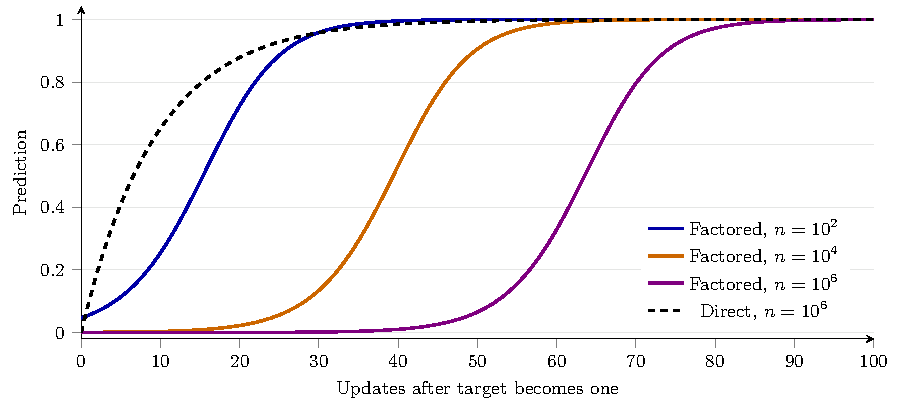
\includegraphics[width=0.85\textwidth]{../figures/lecture21-recovery.pdf}
\caption{Scalar gradient updates with $\eta=0.1$. After $n$ zero targets,
the target is held at one. Longer histories delay the factored learner's
recovery. The direct learner's contraction rate is independent of $n$.
}
\label{fig:recovery}
\end{figure}
\FloatBarrier

\section{Full feedback permits retention without repeated errors}
\label{sec:full-information}

We now work through a fixed-timescale example. With two actions and
complete observations
of their losses, projected gradient descent recovers from every inherited
state and eventually selects a best action with probability one when
the two losses are constant. The proof reuses the online regret argument from Lecture 12, but
applies it after every possible history.
The minimax continuation benchmark $B_T^\star$ has order $\sqrt T$ in
$\cP_{\rm fi}$. We compare projected gradient, Fixed Share, and
shifted-entropy mirror descent (SEMD)
against that benchmark, first on constant losses and then with noise. For a fixed
sufficiently large $C$, we also determine the order of
$F_{\cP_{\rm fi}}(T,C\sqrt T)$.

\subsection{The projected-gradient update}

Use the two-action full-information model and loss in
\cref{eq:mixture-loss}. For a supplied $T\ge1$, set $\eta=T^{-1/2}$,
initialize $X_0=1/2$, and
after observing $Z_{t+1}$ perform
\begin{equation}
 G_{t+1}=Z_{t+1,1}-Z_{t+1,2},\qquad
 X_{t+1}=\Pi_{[0,1]}(X_t-\eta G_{t+1}),
 \label{eq:projected}
\end{equation}
where $\Pi_{[0,1]}(v)=\min\{1,\max\{0,v\}\}$.
The algorithm stores one probability, reads two losses, and performs one
subtraction and clipping operation per round. It needs $T$, but neither a
loss gap nor the environment law. The same update is used during all
inherited histories and future evaluations.

At $X_t=0$, evidence that action one is better still makes $G_{t+1}<0$,
so the next update can restore positive probability to action one.
The feedback remains available even when an action is never selected.

\begin{proposition}[Projected gradient at a fixed timescale]
\label{thm:projected}
Let $\cA_T$ be the algorithm in \cref{eq:projected}.
\begin{enumerate}[(a),leftmargin=*]
\item Its continuation regret satisfies
$\Cont_{\cP_{\rm fi}}^{\cA_T}(T)\le\sqrt T$.
\item Suppose $P=\delta_c$ for a constant loss vector
$c=(c_1,c_2)^\top$ with $c_1\ne c_2$, and put $\Delta=|c_1-c_2|$.
From any inherited state, the learner assigns probability one to the
better action after at most $\lceil1/(\eta\Delta)\rceil$ updates.
Consequently $\Ret_{\delta_c}^{\cA_T,\infty}(K)=0$ for every $K\ge1$.
\item The continuation order is optimal:
$\sqrt T/16\le B_T^\star\le\sqrt T$ for the class $\cP_{\rm fi}$.
\end{enumerate}
\end{proposition}

\begin{proof}
Fix any inherited history and reindex its next $T$ decisions as
$X_0,\ldots,X_{T-1}$. Reindexing is only for the proof; the learner is
not reset. The inherited probability lies in $[0,1]$.
For every comparator $u\in[0,1]$, projection gives
\[
 (X_{t+1}-u)^2
 \le(X_t-\eta G_{t+1}-u)^2
 =(X_t-u)^2-2\eta G_{t+1}(X_t-u)+\eta^2G_{t+1}^2.
\]
The loss difference equals $G_{t+1}(X_t-u)$. Rearranging, summing, and
using $|G_{t+1}|\le1$ yields
\begin{equation}
 \sum_{t=0}^{T-1}\bigl(\ell(X_t,Z_{t+1})-\ell(u,Z_{t+1})\bigr)
 \le\frac{(X_0-u)^2}{2\eta}+\frac{\eta T}{2}
 \le\frac{1}{2\eta}+\frac{\eta T}{2}.
 \label{eq:restart-free-bound}
\end{equation}
The inequality holds for every realized loss sequence. Take expectations,
choose $u$ to minimize $L_P$, and substitute $\eta=T^{-1/2}$.
The bound is independent of the inherited history, proving (a).

For (b), suppose $c_1<c_2$. Each update increases $X_t$ by
$\eta\Delta$, with clipping at one. Thus after $k$ updates from
inherited probability $x$,
\[
 X_k=\min\{1,x+k\eta\Delta\}.
\]
The asserted update bound follows. Once $X_k=1$, all later losses equal
the comparator's loss. The other ordering is symmetric.
If $c_1=c_2$, regret is already zero for every mixture.
Part (c)'s upper bound is (a); the lower bound is proved in
\cref{app:minimax}.
\end{proof}

The learner can stop selecting the worse action under constant losses and
still respond when later observations favor that action. Full feedback
supplies the evidence for correction, and the bounded interval $[0,1]$
limits how far the prediction must move after any history.
\Cref{ex:l21-probability-floor} compares this
learner with a modification that has the same continuation order but
positive tail retention regret on a constant loss vector.

\subsection{Fixed Share pays for permanent mixing}

A second way to control inherited state is to keep a positive weight on
every action. \emph{Fixed Share} first applies an exponential-weights
update, then mixes the result with the uniform action distribution.
For parameters $\eta>0$ and $0<\alpha<1$, initialize
$W_0=(1/2,1/2)^\top$, predict $X_t=W_{t,1}$, and update
\begin{equation}
 \widetilde W_{t+1,i}
 =\frac{W_{t,i}e^{-\eta Z_{t+1,i}}}
        {\sum_{j=1}^2 W_{t,j}e^{-\eta Z_{t+1,j}}},\qquad
 W_{t+1,i}=(1-\alpha)\widetilde W_{t+1,i}+\frac\alpha2.
 \label{eq:fixed-share}
\end{equation}
The two stored weights always sum to one, and each is at least $\alpha/2$.
The floor bounds the amount of new evidence needed to restore a previously
disfavored action. It also forces continued selection of a worse action
when the losses remain constant.

\begin{proposition}[Fixed Share at a fixed timescale]
\label{ex:fixed-share}
For $T\ge2$, choose $\alpha=1/T$ and
$\eta=\sqrt{8(1+\log(2T))/T}$. Then
\[
 \Cont_{\cP_{\rm fi}}^{\rm FS}(T)
 \le\sqrt{\frac{T(1+\log(2T))}{2}}.
\]
For every constant loss vector $c$ with gap $\Delta=|c_1-c_2|>0$,
$\Ret_{\delta_c}^{{\rm FS},\infty}(K)\ge\Delta K/(2T)$.
\end{proposition}
\begin{proof}
Fix any inherited history, reindex the next $T$ rounds from zero, and
choose either comparator action $i$. Define the exponential mixture loss
$M_t=-\eta^{-1}\log\sum_{j=1}^2W_{t,j}e^{-\eta Z_{t+1,j}}$.
Hoeffding's lemma for losses in $[0,1]$ gives
$\ell(X_t,Z_{t+1})\le M_t+\eta/8$.
The update satisfies
$\eta(M_t-Z_{t+1,i})=\log\widetilde W_{t+1,i}-\log W_{t,i}$.
For the first $T-1$ rounds, use
$\widetilde W_{t+1,i}\le W_{t+1,i}/(1-\alpha)$; for the last round,
use $\widetilde W_{T,i}\le1$. Summing telescopes the log weights and gives
\[
 \sum_{t=0}^{T-1}\bigl(\ell(X_t,Z_{t+1})-Z_{t+1,i}\bigr)
 \le\frac{\log(2/\alpha)+(T-1)\log(1/(1-\alpha))}{\eta}
        +\frac{\eta T}{8}.
\]
The initial weight of action $i$ is at least $\alpha/2$, even after an
arbitrary history. Since $(T-1)\log(1/(1-1/T))\le1$, substituting the
parameters and taking expectations proves the continuation bound.
The worse action has weight at least $\alpha/2$ on every round, proving
the retention bound.
\end{proof}

Fixed Share controls recovery, with an extra $\sqrt{\log T}$ factor in
this bound, but pays a positive retention cost even without noise.
Projected gradient already shows that the deterministic cost is avoidable.
The next update gives the same lesson within an entropy-based method.

\subsection{Shifted entropy allows zero weights and recovery}

Ordinary entropy has an unbounded derivative at probability zero. Adding
a positive shift inside the entropy makes its derivative finite on the
whole decision interval. \emph{Shifted-entropy mirror descent}
uses the convex function
\[
 \phi(x)=(x+\tfrac12)\log(x+\tfrac12)
       +(\tfrac32-x)\log(\tfrac32-x),\qquad x\in[0,1],
\]
and its \emph{Bregman divergence}
$D_\phi(u,x)=\phi(u)-\phi(x)-\phi'(x)(u-x)$.
Starting from $X_0=1/2$, the update minimizes the observed linear loss
plus a penalty for changing the current decision:
\begin{equation}
 X_{t+1}=\operatorname*{arg\,min}_{x\in[0,1]}
       \{\eta G_{t+1}x+D_\phi(x,X_t)\},\qquad
 G_{t+1}=Z_{t+1,1}-Z_{t+1,2}.
 \label{eq:semd}
\end{equation}
There is a simple scalar implementation. Put $a=\log3$ and store
$\Theta_t=\phi'(X_t)=\log((X_t+1/2)/(3/2-X_t))$. Then
\[
 \Theta_{t+1}=\Pi_{[-a,a]}(\Theta_t-\eta G_{t+1}),\qquad
 X_{t+1}=\frac{2e^{\Theta_{t+1}}}{1+e^{\Theta_{t+1}}}-\frac12.
\]
The algorithm adds evidence in the transformed coordinate and clips it to
a bounded interval. The two endpoints correspond to probabilities zero
and one. Evidence favoring the other action moves the coordinate back
into the interval, so a zero probability can recover.

\begin{proposition}[SEMD at a fixed timescale]
\label{ex:semd}
For $\eta=T^{-1/2}$, the update in \cref{eq:semd} satisfies
\[
 \Cont_{\cP_{\rm fi}}^{\rm SEMD}(T)
 \le(\log3+1/4)\sqrt T.
\]
On a constant loss vector with gap $\Delta>0$, SEMD reaches the better
action's endpoint after at most $\lceil2\log3/(\eta\Delta)\rceil$
updates from any inherited state. Thus
$\Ret_{\delta_c}^{{\rm SEMD},\infty}(K)=0$ for every $K\ge1$.
\end{proposition}
\begin{proof}
Direct differentiation gives $\phi''(x)\ge2$ and
$D_\phi(u,x)\le a$ for $u,x\in[0,1]$. The optimality condition in
\cref{eq:semd}, together with $D_\phi(v,x)\ge(v-x)^2$, gives
\[
 \eta G_{t+1}(X_t-u)
 \le D_\phi(u,X_t)-D_\phi(u,X_{t+1})
        +\frac{\eta^2G_{t+1}^2}{4}.
\]
Summing over the next $T$ rounds bounds regret by $a/\eta+\eta T/4$,
uniformly over the starting state. Under constant losses, the transformed
coordinate moves by $\eta\Delta$ toward the better endpoint until it
reaches that endpoint and remains there.
\end{proof}

The shift changes the geometry of the update without imposing a positive
action probability. Full feedback supplies the evidence needed to reverse
a decision even at the boundary. Fixed Share preserves recovery by
continually assigning positive probability to both actions. SEMD preserves
recovery by keeping the transformed coordinate bounded, so it can assign
zero probability to the worse action and incur zero persistent cost on
constant losses.

\subsection{Adaptation to an unknown noise level}
\label{sec:noise-adaptation}

A useful learner should incur less persistent error when its observations
are more reliable. For the two-action problem, the relevant noise is in
the \emph{loss difference}. Under a fixed $P\in\cP_{\rm fi}$, define
\[
 V=Z_2-Z_1,\qquad \Delta=|\E[V]|,\qquad
 \sigma^2=\E[(V-\E[V])^2].
\]
Common noise added to both losses cancels from $V$. The algorithm observes
$V$ through the full loss vector; it is not given $\Delta$ or $\sigma^2$.

\begin{proposition}[Noise-sensitive recovery and retention]
\label{ex:noise-sensitive}
For projected gradient with any fixed $\eta>0$, every inherited history
$h$ and every integer $m\ge1$ satisfy
\begin{equation}
 R_P^{\rm PG}(h,m)
 \le\frac1{2\eta}+\frac{\eta m\sigma^2}{2}+\Delta.
 \label{eq:pg-noise}
\end{equation}
Projected gradient and scalar SEMD have persistent coefficients
\begin{equation}
 \rho_P^{\rm PG}\le\frac{\eta\sigma^2}{2},\qquad
 \rho_P^{\rm SEMD}\le\frac{\eta\sigma^2}{4}.
 \label{eq:noise-retention}
\end{equation}
\end{proposition}

\Cref{app:noise-adaptation} proves these bounds by tracking the first two
moments of the distance from the better action. The same updates work at
every noise level: their retention bounds scale with $\sigma^2$, and
their persistent cost is zero when $\sigma^2=0$.
In contrast, the action-probability floor in Fixed Share causes a positive
cost even when $\sigma^2=0$ and $\Delta>0$.

The worst-case tradeoff remains useful as a common constraint on these
instance-sensitive guarantees. It asks how much retention error some
noisy environment must cause when recovery is uniformly fast.

\begin{proposition}[Optimal retention cost at the natural continuation scale]
\label{prop:natural-cost}
For each fixed $C\ge8$, as $T\to\infty$ through integer values,
\[
 F_{\cP_{\rm fi}}(T,C\sqrt T)=\Theta_C(T^{-1/2}),
\]
where the positive constants may depend on $C$.
\end{proposition}

Any algorithm with $\Cont_{\cP}^{\cA}(T)\le B$ satisfies
$\rho_P^\cA\le B/T$: partition a retention evaluation into $T$-round
blocks and a remainder shorter than $T$. Consequently projected gradient
and scalar SEMD both attain the upper order in
\cref{prop:natural-cost}. The lower bound in \cref{app:retention-cost}
uses noisy laws that depend on $T$. The variance-sensitive bounds in
\cref{eq:noise-retention} give tighter retention guarantees when the
loss-difference variance is smaller.

\Cref{ex:l21-noisy-mean} gives a related calculation for mean estimation:
a fixed stepsize gives recovery independent of the number of preceding
steps and persistent error proportional to the observation variance.
The running mean has vanishing error in a persistent environment, but after
$n$ old observations and $k$ new ones its old mean still has weight
$n/(n+k)$. Halving an inappropriate inherited bias requires $k=n$.
Thus decreasing the stepsize with elapsed training can destroy uniform
recovery even as it improves estimation in one environment.

\section{Choosing a gain for a noisy autoregressive process}
\label{sec:stepsize-aggregation}

In the AR(1) model of \cref{eq:ar-model}, the best update size depends on
the unknown innovation and measurement-noise variances $q$ and $r$. A large update follows the signal
quickly but also follows measurement noise. A small update suppresses
measurement noise but uses less of the new information about the signal.
We will aggregate filters with different update sizes and compare their
prediction errors. The observations in this example can be correlated, and
the comparison is with a learning algorithm: a filter that continues to
update its prediction.

\subsection{The best fixed gain}

For a \emph{gain} $\eta\in[0,1]$, initialize $X_0^{(\eta)}=0$ and use
\begin{equation}
 X_{t+1}^{(\eta)}
 =\gamma\bigl((1-\eta)X_t^{(\eta)}+\eta Y_{t+1}\bigr).
 \label{eq:ar-filter}
\end{equation}
The filter first combines its prediction with the new measurement, then
applies the known dynamics to predict the next state. Its predictions
remain in $[-1/2,1/2]$. The gain is the stepsize of the correction toward
the measurement.

\begin{proposition}[The noise levels determine the best gain]
\label{ex:ar-risk}
The limiting mean squared prediction error of \cref{eq:ar-filter} is
\begin{equation}
 L_\infty(\eta)
 :=\lim_{t\to\infty}\E[(X_t^{(\eta)}-S_t)^2]
 =\frac{q+\gamma^2\eta^2r}{1-\gamma^2(1-\eta)^2}.
 \label{eq:ar-risk}
\end{equation}
For $q,r>0$, the unique minimizing gain $\eta^\star\in(0,1)$ satisfies
\begin{equation}
 \gamma^2r(\eta^\star)^2+
 \bigl(r(1-\gamma^2)+q\bigr)\eta^\star-q=0.
 \label{eq:ar-optimal-gain}
\end{equation}
For $q=0$, gain zero is optimal; for $r=0$, gain one is optimal.

Write $\delta=1-\gamma^2$ and let
$L^\star=\min_{\eta\in[0,1]}L_\infty(\eta)$ be the optimal limiting error.
For $q,r>0$,
\begin{equation}
 L^\star=\frac{q-\delta r+\sqrt{(\delta r-q)^2+4qr}}2,
 \qquad \eta^\star=\frac{L^\star}{L^\star+r}.
 \label{eq:ar-optimal-error}
\end{equation}
The optimal error and gain have three regimes:
\begin{center}
\renewcommand{\arraystretch}{1.3}
\begin{tabular}{lll}
\toprule
Noise variances & Optimal error $L^\star$ & Optimal gain $\eta^\star$\\
\midrule
$q\le\delta^2r$ & $\asymp q/\delta$ & $\asymp q/(\delta r)$\\
$\delta^2r\le q\le r$ & $\asymp\sqrt{qr}$ & $\asymp\sqrt{q/r}$\\
$q\ge r$ & $\asymp q$ & $\asymp1$\\
\bottomrule
\end{tabular}
\end{center}
Here $\asymp$ means upper and lower bounds by positive constant multiples,
with constants independent of $\gamma,q,r$.
\end{proposition}
\begin{proof}
Subtract the signal update from the filter update:
\[
 X_{t+1}^{(\eta)}-S_{t+1}
 =\gamma(1-\eta)(X_t^{(\eta)}-S_t)
   +\gamma\eta\varepsilon_{t+1}-U_{t+1}.
\]
Independence and zero means eliminate the cross terms. The mean squared
error therefore obeys a scalar affine recursion with contraction factor
$\gamma^2(1-\eta)^2<1$ and additive term $\gamma^2\eta^2r+q$.
Its limit is \cref{eq:ar-risk}. Differentiating the ratio gives
\cref{eq:ar-optimal-gain}; its left side increases from $-q$ to $r$
as $\eta$ runs from zero to one. The boundary cases follow directly
from \cref{eq:ar-risk}.

At the minimizing gain, differentiation also gives
$\eta^\star r=(1-\eta^\star)L^\star$. Substituting this relation into
\cref{eq:ar-risk} yields
\[
 (L^\star)^2+(\delta r-q)L^\star-qr=0.
\]
The positive root gives \cref{eq:ar-optimal-error}. Substitution into this
quadratic brackets its positive root between $q/(2\delta)$ and
$q/\delta$ in the first regime, between $\sqrt{qr}/2$ and
$2\sqrt{qr}$ in the second, and between $q$ and $2q$ in the third.
The gain estimates follow from $\eta^\star=L^\star/(L^\star+r)$.
\end{proof}

The three regimes explain what limits prediction. When
$q\le\delta^2r$, measurements are sufficiently noisy that predicting zero
already gives the optimal order $q/\delta$, the limiting signal variance.
In the middle regime, correcting toward new measurements balances tracking
the signal against suppressing measurement noise, giving error
$\sqrt{qr}$. When $q\ge r$, the new innovation is the main source of error:
even an exact observation of $S_t$ leaves variance $q$ when predicting
$S_{t+1}$.

For fixed $\gamma$, the optimal gain therefore depends on the unknown
ratio $q/r$. Estimating the variances is one way to tune the filter.
Aggregation offers another: compare gains by their observed prediction
losses.

\subsection{A finite grid and its aggregation guarantee}

The persistence coefficient determines a sufficient range of gains.
Define the grid
\begin{equation}
 J=\max\left\{0,\left\lceil\log_2\frac{\gamma^2}{1-\gamma^2}
                         \right\rceil\right\},\qquad
 \cH=\{0,2^{-J},2^{-J+1},\ldots,1\},\qquad M=J+2.
 \label{eq:gain-grid}
\end{equation}
For example, $\gamma=0.99$ gives eight gains:
$0,1/64,1/32,1/16,1/8,1/4,1/2,1$.
The smallest positive gain is chosen so that still smaller optimal gains
can be approximated by gain zero. The dyadic spacing approximates the
remaining gains. For every $q,r\ge0$ allowed by the model,
\begin{equation}
 \min_{\eta\in\cH}L_\infty(\eta)
 \le2\min_{\eta\in[0,1]}L_\infty(\eta).
 \label{eq:gain-grid-comparison}
\end{equation}
Thus the grid covers the unknown noise ratio with a specified error factor.

Enumerate the gains as $\eta_1,\ldots,\eta_M$ and run all $M$ filters.
Fix an integer comparison timescale $T\ge2$. Initialize weights
$W_{0,j}=1/M$ and predict $X_t=\sum_jW_{t,j}X_t^{(\eta_j)}$.
After observing $Y_{t+1}$, compute the half-squared losses
$A_{t+1,j}=\tfrac12(X_t^{(\eta_j)}-Y_{t+1})^2$ and apply Fixed Share:
\begin{equation}
 \widetilde W_{t+1,j}
 =\frac{W_{t,j}e^{-A_{t+1,j}}}{\sum_iW_{t,i}e^{-A_{t+1,i}}},\qquad
 W_{t+1,j}=(1-1/T)\widetilde W_{t+1,j}+\frac1{MT}.
 \label{eq:filter-aggregation}
\end{equation}
Update every filter using \cref{eq:ar-filter}, including filters with small
weights. The aggregate stores $M$ predictions and $M$ weights and uses
$O(M)$ operations per observation. Its inputs are $\gamma$ and $T$;
the variances $q,r$ are unknown.

\begin{proposition}[Adaptation to the unknown noise ratio]
\label{ex:filter-aggregation}
For the filter aggregate in \cref{eq:filter-aggregation},
\begin{equation}
 \begin{aligned}
 \limsup_{N\to\infty}\frac1N\sum_{t=0}^{N-1}\E[(X_t-S_t)^2]
 &\le \min_{\eta\in\cH}L_\infty(\eta)+\frac{2(\log(MT)+1)}T\\
 &\le 2\min_{\eta\in[0,1]}L_\infty(\eta)+\frac{2(\log(MT)+1)}T.
 \end{aligned}
 \label{eq:filter-oracle}
\end{equation}
\end{proposition}

The comparison is with the best fixed gain chosen with knowledge of the
noise variances. As $T$ grows, the aggregate's upper bound on excess error
relative to the best supplied filter tends to zero; the grid gives a
factor-two comparison with every fixed gain. The reason observed losses
suffice is the identity
\[
 \E[(X_t-Y_{t+1})^2]=\E[(X_t-S_t)^2]+r,
\]
which also holds for each filter. Fresh measurement noise adds the same
quantity to every expected squared prediction loss.

For squared loss, cumulative excess loss relative to a filter can be
bounded logarithmically in the number of filters. On the prediction range,
$x\mapsto e^{-(x-y)^2/2}$ is concave. Applying this concavity to the
weighted mean prediction gives
\[
 \tfrac12(X_t-Y_{t+1})^2
 \le -\log\sum_{j=1}^M W_{t,j}e^{-A_{t+1,j}}.
\]
The right side can be summed using the same weight-update identity as in
the Fixed Share proof. Over any next $T$ rounds, the aggregate's cumulative
half-squared observed loss exceeds that of any one filter by at most
$\log(MT)+1$, independently of the preceding history.
\Cref{app:filter-aggregation} proves this block bound and the grid comparison.

\subsection{How much can choosing among gains help?}

The improvement over a single gain chosen without the noise variances can
be arbitrarily large. A persistent signal makes the choice particularly
consequential: small gains suppress noisy measurements, while large gains
use accurate measurements to track new innovations.

\begin{proposition}[An arbitrarily large improvement over a preset gain]
\label{ex:ar-preset-gain}
Let $\delta=1-\gamma^2\in(0,1/2]$. Use the grid in
\cref{eq:gain-grid}, with
$M=|\cH|=2+\lceil\log_2((1-\delta)/\delta)\rceil$ filters.
Thus $\gamma$ determines $M$. Choose an integer $T\ge2$ such that
\begin{equation}
 \frac{2(\log(MT)+1)}T\le\frac{\delta^2}{64}.
 \label{eq:ar-comparison-timescale}
\end{equation}
For every single gain $\eta\in[0,1]$ fixed before observing data, using
only $\gamma,T$, there are positive noise variances allowed by \cref{eq:ar-model}
for which the Fixed Share aggregate satisfies
\begin{equation}
 \overline L_{\rm agg}
 :=\limsup_{N\to\infty}\frac1N\sum_{t=0}^{N-1}\E[(X_t-S_t)^2]
 \le 7\delta L_\infty(\eta).
 \label{eq:ar-preset-comparison}
\end{equation}
\end{proposition}

Thus the single gain's limiting error can exceed the aggregate's long-run
average error by a factor at least $1/(7(1-\gamma^2))$, which grows without
bound as $\gamma\to1$. \Cref{app:filter-aggregation} proves the claim
using two settings: accurate measurements that favor a large gain, and
noisy measurements that favor a small gain. For each fixed $\gamma$ and
chosen $T$, the aggregate uses the same grid and timescale on both noise
settings. The condition on $T$ keeps
the additional error in the aggregation bound small enough to obtain the
stated improvement.\endnote{When $\gamma$ is unknown, the same aggregation rule can
compare filters with different persistence coefficients and gains.
\Cref{app:unknown-persistence} gives the construction and its comparison
bound.}
\label{en:unknown-persistence}

Each filter updates its prediction as observations arrive. The aggregate
therefore compares $M$ update rules without discretizing all possible
prediction values. The same construction can compare copies of a learning
algorithm that use different stepsizes, at the cost of maintaining and
updating one state per copy.
For a convex loss in the prediction, a mixture's loss is at most the
weighted average of the copies' losses. The aggregation rule updates its
weights using all copies' losses on each new example. In the two-action
full-information problem, SEMD bounds the additional loss relative to any
copy uniformly over preceding histories.
\endnote{\Cref{app:stepsize-aggregation} gives the SEMD update over
projected-gradient copies and its continuation bound. On constant losses,
the aggregate has zero tail retention because each copy eventually incurs
zero excess loss.}
\label{en:stepsize-aggregation}

\section{Bandit feedback requires continued testing}
\label{sec:bandit-testing}

With \emph{bandit feedback}, the learner observes only its chosen action's
loss. An action that is never selected supplies no evidence about its
quality. The following two environments show that preserving the ability
to detect the better action requires continued testing, even when every
observed loss is noiseless.

Consider the two constant loss vectors
\[
 c^-=(1/2,1)^\top,\qquad c^+=(1/2,0)^\top.
\]
Take $\cX=\{1,2\}$ and $\cZ=[0,1]$. The learner's decision is an action
$A_t\in\cX$, and its observation is $Z_{t+1}=c_{A_t}$ for the fixed environment
$c\in\{c^-,c^+\}$. The history is
$H_t=(A_0,Z_1,\ldots,A_{t-1},Z_t)\in\cH_t$, where
$\cH_t=(\{1,2\}\times[0,1])^t$. The learner specifies a next-action
distribution at every such history.
For fixed $c$, the continuation measure $\P_{h,\cA}$ starts from $h$
and uses this action-dependent observation rule. Local regret is
\[
 R_c^\cA(h,T)=\E_{h,\cA}\!\left[\sum_{t=0}^{T-1}
       (c_{A_{n+t}}-\min_i c_i)\right],\qquad h\in\cH_n.
\]
Continuation takes the supremum over $h$ and $c\in\{c^-,c^+\}$;
retention uses histories generated in one fixed environment, with the same
averaging and limits as in \cref{def:retention,eq:retention-coefficient}.
The two environments give identical observations whenever the learner
selects action one. Comparing them isolates the cost of obtaining
information about an unchosen action.

\begin{proposition}[Necessary and sufficient testing]
\label{ex:bandit-pair}
Suppose $\Cont_{\{c^-,c^+\}}^\cA(T)\le B$, where $B>0$, and put
$r=\lceil4B\rceil$. If $r\le T$, then
\[
 \rho_{c^-}^\cA\ge\frac1{4r}.
\]
Conversely, for every integer $q\ge2$, there is a periodic-testing learner
with
\[
 \Cont_{\{c^-,c^+\}}^{\rm test}(T)
 \le\frac12\max\{q,1+\lceil T/q\rceil\},\qquad
 \rho_{c^-}^{\rm test}=\frac1{2q},\qquad \rho_{c^+}^{\rm test}=0.
\]
\end{proposition}
\begin{proof}
Fix any inherited history. Under $c^+$, selecting action one for all next
$r$ rounds incurs regret $r/2$. The continuation bound therefore makes the
probability of that event at most $2B/r\le1/2$. Until action two is
selected, the observed losses are identical under $c^-$ and $c^+$.
Hence action two is selected within the next $r$ rounds with probability
at least $1/2$ under $c^-$ as well. Each such selection costs excess loss
$1/2$, giving expected regret at least $1/4$ on every $r$-round block.
Summing blocks gives $\rho_{c^-}^\cA\ge1/(4r)$.

For the upper bound, keep a preferred action, initially one. Select action
two at every step whose index is a multiple of $q$, and otherwise select
the preferred action. Whenever action two is selected, set the preferred
action to two if its observed loss is less than $1/2$, and to one otherwise.
Under $c^+$, within $q$ rounds a selection of action two makes all later
choices correct. Under $c^-$, a wrong inherited preference is corrected
on its first use, and at most $\lceil T/q\rceil$ scheduled tests occur
in the block. These counts prove the continuation bound. In the persistent
$c^-$ instance, exactly one round in every $q$ tests the worse action;
in $c^+$, all choices are eventually correct.
\end{proof}

Taking $q=\lceil\sqrt T\rceil$ for $T\ge4$ gives continuation
$O(\sqrt T)$ and worst persistent cost $\Theta(T^{-1/2})$.
The lower bound shows that every learner with an $O(\sqrt T)$
continuation guarantee pays this order on $c^-$. Under full feedback,
one observation identifies the better action in either instance and tail
retention is zero. Under bandit feedback, preserving the ability to detect
the other instance requires recurring tests of a known worse action.

An open extension of this calculation is to characterize the optimal
retention cost for stochastic bandits as a joint function of the
continuation budget, the loss gaps, and the noise levels, using algorithms
that know neither the gaps nor the noise levels. The noiseless pair shows
why such a characterization must include the cost of obtaining information
about an unchosen action, even at zero observation noise.

\section{Implications for continued training and memory}
\label{sec:implications}

The examples separate properties that a useful learning system must combine.
A rich prediction class supplies possible behaviors. The inherited state
and update rule determine which of those behaviors the learner can reach
quickly. The observation interface determines whether the evidence needed
for a correction becomes available.

For a new training stage, initial performance is therefore only part of
the evaluation. The factored example can have excellent performance on its
preceding objective while the resulting small factors delay subsequent
updates. In reinforcement learning, inherited action probabilities also
affect which training observations the system obtains. These dependencies
help explain why the objective, parameterization, optimizer state, and
data-collection rule should be considered together.

For a runtime with memory, the same questions concern retrieval and revision.
An old record can remain useful indefinitely; an incorrect record can also
continue to influence the system. The relevant design question is whether
available corrective evidence can change the resulting decisions within
a useful timescale, while reliable records continue to improve performance.

\section{Take-home messages}
\begin{enumerate}[leftmargin=*]
\item Plasticity is the ability to make effective use of new information;
stability is the ability to make effective use of past information.
Together they ask the learner to use all available information, new and old.
Partial information and limited representation can make further learning
useful under fixed environmental laws.
\item The learning system includes every state variable that affects future
behavior. Frozen trained components can participate in a plastic system
through mutable runtime memory.
\item A single learner cannot have sublinear history-uniform continuation
regret at every horizon, even for stationary noisy full-information
observations. Choose an adaptation timescale before comparing retention
under a common continuation requirement.
\item Eventual convergence after every finite training history can coexist
with linear worst-case continuation regret. The factored scalar learner
demonstrates this distinction with the same prediction class as a learner
that recovers uniformly quickly.
\item In the two-action full-information model, projected gradient and
SEMD attain optimal-order continuation and zero tail retention on constant
deterministic losses. Fixed Share over actions pays a permanent mixing
cost on those instances.
\item Under noisy full-information observations, the optimal worst-case
persistent excess-loss coefficient is of order $T^{-1/2}$ when the
continuation budget is a fixed sufficiently large multiple of $\sqrt T$.
Projected gradient and SEMD also have retention bounds proportional to
the loss-difference variance, without knowing that variance.
\item In the noisy AR(1) model, the best filter gain depends on the ratio
of innovation to measurement variance. Aggregating a finite grid of filters
competes with that tuned choice using observable prediction losses. For
increasingly persistent signals and sufficiently long comparison timescales,
the improvement over any single gain chosen without the variances can be
arbitrarily large.
\item Bandit feedback can require persistent testing of a worse action
even on noiseless instances. The two-instance example gives matching
orders for the cost of maintaining this ability to obtain information.
\end{enumerate}

\printendnotes

\section*{Bibliographical notes}

\paragraph{Fixed environments and limited learners.}
\citet{kumar2024} develop the small-agent, big-world motivation and
propose criteria for environments in which limited agents must continue
learning. \citet{wen2025} study linear-Gaussian sequential prediction under
a mutual-information constraint on retained state. The information constraint
relaxes a hard finite-memory restriction.

\paragraph{Continuation and retention.}
The definitions and comparison in \cref{sec:framework} specialize the
instructor's working manuscript \emph{Continuation and Retention Regret:
A Theory of Stability and Plasticity} to i.i.d.\ observations and fixed
decision comparators. The general formulation allows an environment whose
conditional observation law depends on the history and current action.
Learner and comparator then continue from the same inherited history and
induce their own future trajectories.
The main text uses $K$ where the manuscript uses $L$ for retention-window
length, preserving the course convention for population risk.

The manuscript states the all-timescale impossibility for a class of fixed
full-information loss sequences. \Cref{thm:no-all-scales} proves the same
timescale obstruction within the lecture's i.i.d.\ model, using one
deterministic law and one noisy law. Its proof makes explicit the recurring
cost of responding to misleading observations.

The manuscript's positive full-information result uses shifted-entropy
mirror descent for an arbitrary number of actions. The two-action
projected-gradient proof in \cref{thm:projected} uses the standard
online-gradient inequality developed in Lecture 12.
The comparison in \cref{ex:fixed-share,ex:semd} specializes the manuscript's
Fixed Share and SEMD results. Fixed Share originates with
\citet{herbster1998}; the shifted-entropy expert update is developed by
\citet{buchbinder2012}. Both updates extend to more than two actions.
The lower bound in \cref{app:minimax} is the usual two-distribution
testing argument.

\Cref{prop:natural-cost} and its finite lower bound specialize the
instructor's accompanying research note, \emph{The optimal retention cost
of uniform continuation guarantees} (2026), developed during preparation
of this lecture. The note studies the dependence on the continuation budget
and other losses, including
squared loss. Those results use additional algorithms and testing arguments.

The variance-sensitive clipping calculation in
\cref{app:noise-adaptation} and the noiseless bandit pair in
\cref{ex:bandit-pair} were developed for these notes. The bandit example
isolates the continued-testing mechanism in the working manuscript.
The scalar factorization example and the compatible ReLU exercise are
elementary constructions developed for these notes.

\paragraph{Selecting learning rates and filter gains.}
\Cref{app:stepsize-aggregation} applies SEMD to learning algorithms as
experts. Aggregating projected-gradient instances with different stepsizes
is the central construction in the Ader algorithm of \citet{zhang2018},
which controls dynamic regret against moving comparators.
MetaGrad, developed by \citet{vanerven2021}, combines multiple learning
rates with specially designed surrogate losses. Its guarantees adapt to
curvature, gradient magnitudes, and stochastic Bernstein conditions.
The Squint algorithm of \citet{koolen2015} gives second-order expert bounds
in terms of cumulative squared excess losses. These guarantees account
for quantities absent from the worst-case $2\sqrt{T\log(M+1)}$
aggregation bound in \cref{app:stepsize-aggregation}.

The noisy AR(1) example is a scalar state-space prediction problem.
\citet{kalman1960} derives recursive linear estimation from error
covariances. For the Gaussian version of \cref{eq:ar-model}, the optimal
constant gain in \cref{eq:ar-optimal-gain} is the steady-state Kalman
gain. The bounded model used here permits a direct Fixed Share comparison
under squared loss. The dyadic gain grid, its factor-two comparison, and
the two-setting comparison with a preset gain were derived for these notes.
Aggregation uses prediction
losses to select among gains without estimating the process and measurement
variances separately.

\paragraph{Plasticity in neural networks.}
\citet{dohare2024} document declining performance on subsequent learning
problems and investigate selective unit reinitialization in supervised and
reinforcement-learning experiments.
\citet{farias2025} analyze a single ReLU with an adversarially chosen target
and an idealized reset oracle. Their positive theorem uses population
gradients, an activation oracle, and specified initialization and target
conditions.
\citet{lewandowski2025} give positive theoretical results for linear and
restricted diagonal deep-linear models, together with experiments on deep
Fourier features. Their assumptions and convergence criteria differ from
the history-uniform finite-timescale requirement in these notes.

\paragraph{Offline pretraining followed by online learning.}
\citet{nakamoto2023} study deterioration of a competent offline-trained
policy during online fine-tuning. Conservative offline estimation discourages
high values for actions poorly supported by the data. Excessive pessimism
can subsequently make inferior actions look preferable as fresh evaluations
arrive. Calibrated Q-learning (Cal-QL) modifies the conservative penalty:
its downward pressure stops below a reference-policy value, while the
Bellman-fitting loss remains. The paper gives experiments and theory for
idealized fitted-value iteration under structural and statistical
assumptions.

The broader lesson is that a trained state should support useful subsequent
updates as well as good current decisions. The scalar example concerns
small parameter derivatives; Cal-QL concerns inherited value calibration.
The continuation criterion can evaluate either mechanism once the interface
and comparator are specified.

A related objective-design result is \citet{farebrother2024}, who replace
squared-error value regression with categorical cross-entropy and study
performance across several reinforcement-learning domains, including
robotic manipulation. Their plasticity experiments include changing target
magnitudes. Those empirical findings concern a different mechanism from
Cal-QL's calibration of conservative values.

\section*{Glossary}
\begin{description}[style=nextline,leftmargin=1.5em,labelindent=0pt]
\item[Plasticity]
The ability to incorporate new information and use it to improve decisions;
continuation regret specifies a quantitative requirement from every
inherited history.
\item[Stability and retention]
The ability to keep making effective use of past information. Retention
regret evaluates future performance after the learner's own history in a
persistent environment.
\item[Continual learning]
Learning over an extended sequence of experience while maintaining the
ability to use both new and past information effectively.
\item[Interaction history $H_n$ and inherited history $h$]
The sequence $H_n=(X_0,Z_1,\ldots,X_{n-1},Z_n)$ records the learner's
decisions and observations. A fixed $h\in\cH_n$ is the starting input
to the same decision rule $\cA(\cdot\mid h)$ in a continuation experiment.
The future evaluation boundary is not supplied to the learner.
\item[Continuation law $\P_{h,\cA}$ and expectation $\E_{h,\cA}$]
The probability measure and expectation operator for continuing $\cA$
from a fixed history $h$, with the environment law $P$ held fixed and
implicit in the notation. Retention averages under $\P_{\varnothing,\cA}$.
\item[Local regret $R_P^\cA(h,T)$]
Expected excess cumulative loss over the next $T$ rounds after history $h$,
relative to a best fixed decision for the future environment $P$.
\item[Continuation regret $\Cont_{\cP}^{\cA}(T)$]
The worst local regret over environments in $\cP$ and all finite inherited
histories, at the selected adaptation timescale $T$.
\item[Adaptation timescale $T$]
The future evaluation length at which uniform recovery is required.
A learner may be designed for $T$ while running for an arbitrary lifetime;
the start of an evaluation is not announced.
\item[Retention profile $\Ret_P^\cA(n,K)$]
Local regret averaged over the history generated by running the learner for
$n$ rounds in $P$, followed by $K$ more rounds in the same environment.
\item[Tail retention $\Ret_P^{\cA,\infty}(K)$]
The upper limit of retention regret as the preceding step count $n$ tends to infinity with
evaluation length $K$ fixed.
\item[Factored scalar parameterization]
The map $\theta\mapsto\theta_1\theta_2$ from two scalar parameters to
their predicted value.
Gradient descent updates the two factors separately;
with equal initial factors, their common value is denoted by $\vartheta_t$.
\item[Minimax continuation benchmark $B_T^\star$]
The smallest achievable worst-case continuation regret at timescale $T$
under the specified information and resource constraints.
\item[Persistent excess-loss coefficient $\rho_P^\cA$]
The upper limit of tail retention regret divided by its evaluation length
$K$, as $K$ tends to infinity.
\item[Optimal worst-case retention cost $F_{\cP}(T,B)$]
The infimum of $\sup_{P\in\cP}\rho_P^\cA$ over algorithms whose
continuation regret at timescale $T$ is at most $B$.
\item[Constant-target class $\cP_{\rm const}$]
The laws $\delta_z$, $z\in[0,1]$, supplying one fixed scalar target at every
round. Predictions lie in $[0,1]$ and incur half-squared loss.
\item[Full-information class $\cP_{\rm fi}$]
All probability laws on $[0,1]^2$, supplying i.i.d.\ two-action loss vectors
that the learner observes in full.
\item[Fixed Share]
An exponential-weights update followed by mixing with a fixed uniform
distribution, which keeps every expert's weight positive.
\item[Shifted-entropy mirror descent (SEMD)]
A mirror-descent update using the entropy of positively shifted weights.
Its derivative remains finite at zero probability, permitting
both zero weights and subsequent recovery.
\item[Bregman divergence]
For differentiable convex $\Phi$, the displacement penalty
$D_\Phi(v,w)=\Phi(v)-\Phi(w)-\langle\nabla\Phi(w),v-w\rangle$.
\item[Filter gain]
The correction weight $\eta$ in
$X_{t+1}=\gamma((1-\eta)X_t+\eta Y_{t+1})$ for the noisy AR(1) model.
The innovation variance $q$ describes new latent-state variation, and the
measurement variance $r$ describes observation noise.
The persistence coefficient is $\gamma$; $\delta=1-\gamma^2$ controls the
boundaries between the three optimal-error regimes.
\item[Aggregation of learning algorithms]
Treating continuously updated learners as experts, scoring their
predictions on each observation, and combining the predictions with
adaptively updated weights.
\item[Full-information feedback]
Observation of every action's loss after each round, including unchosen
actions. In this lecture, the law generating those losses is not supplied
to the learner.
\item[Bandit feedback]
Bandit feedback supplies only the chosen action's loss.
\end{description}

\section{Exercises}
\label{sec:exercises}
The exercises examine gradient failure on jointly realizable examples,
the effect of noise on mean estimation, and the retention cost of forcing
every action to have positive probability.
\exerciseinstructions
\setcounter{courseexercise}{0}
\begin{exercisechunk}
\item \textbf{Loss of plasticity with compatible examples.}
\label[exercise]{ex:l21-compatible-relu}
\exerciseprofile{2}{2}{2}{\exproof\quad\excalculation\quad\exinterpretation}{%
Separate the existence of a common predictor from the ability of gradient updates to reach it.}
Consider $f_{a,b}(x)=\max\{ax+b,0\}$ and the loss
$\tfrac12(f_{a,b}(x)-y)^2$. Initialize $(a,b)=(0,1)$ and apply gradient
descent to each presented example with stepsize $\eta=2/5$.
\begin{enumerate}[(a)]
\item Show that one update on $(x,y)=(1,0)$ gives
$(a,b)=(-2/5,3/5)$. Show that subsequent training only on $(2,1)$ leaves
these parameters unchanged, with loss $1/2$ on every round.
\item Exhibit parameters that fit both $(1,0)$ and $(2,1)$ exactly.
Explain why part (a) is a failure of the update dynamics rather than
incompatibility of the two examples. Also compare the future loss with
that of the prescribed initialization on $(2,1)$.
\item Suppose the same two examples are instead drawn independently
forever, with $\P((X,Y)=(1,0))=q$ and
$\P((X,Y)=(2,1))=1-q$, where $0<q<1$.
Prove that the expected one-round loss converges to $(1-q)/2$,
although a predictor with zero population loss exists.
\end{enumerate}
\begin{hints}
For (c), examine the first occurrence of $(1,0)$ and then track
$a+b$ and $2a+b$. Each example occurs infinitely often almost surely.
\end{hints}
\end{exercisechunk}

\begin{exercisechunk}
\item \textbf{Recovery and retention when estimating a noisy mean.}
\label[exercise]{ex:l21-noisy-mean}
\exerciseprofile{2}{2}{3}{\exproof\quad\excalculation\quad\exinterpretation}{%
Distinguish recovery from inherited bias from the persistent cost of noisy updates.}
Let $Y_1,Y_2,\ldots$ be i.i.d.\ in $[0,1]$, with mean $\mu$ and variance
$\sigma^2$. Use $\ell(x,y)=\tfrac12(x-y)^2$, whose best fixed predictor
is $\mu$. Let $\cP$ contain all laws on $[0,1]$.
\begin{enumerate}[(a)]
\item From a deterministic inherited value $x_0\in[0,1]$, set $X_0=x_0$ and use
$X_{k+1}=(1-\eta)X_k+\eta Y_{k+1}$ with $0<\eta\le1$.
Show that
\[
 \E[(X_k-\mu)^2]
 =(1-\eta)^{2k}(x_0-\mu)^2+
 \frac{\eta\sigma^2}{2-\eta}\bigl[1-(1-\eta)^{2k}\bigr].
\]
\item Let $\cA_\eta$ run this update continuously from a fixed initial
value in $[0,1]$. Prove
\[
 \operatorname{Cont}_{\cP}^{\cA_\eta}(T)
 \le\frac{1}{2\eta(2-\eta)}+\frac{T\eta}{8(2-\eta)},
 \qquad
 \operatorname{Ret}_P^{\cA_\eta,\infty}(K)=
 \frac{K\eta\sigma^2}{2(2-\eta)}.
\]
Deduce continuation of order $\sqrt T$ with $\eta=T^{-1/2}$.
\item Consider instead the running sample mean after at least one
observation; before the first observation, predict any fixed value in $[0,1]$.
Show that an inherited history with $n\ge1$ zero observations, followed by
constant target one, gives next-$T$-round regret
\[
 \frac12\sum_{k=0}^{T-1}\left(\frac{n}{n+k}\right)^2.
\]
Deduce $\operatorname{Cont}_{\cP}^{\rm mean}(T)=T/2$ and show that
$\operatorname{Ret}_P^{{\rm mean},\infty}(K)=0$ for every $P\in\cP$ and fixed $K$.
\item Compare the two methods using the criteria in (b)--(c).
Identify which term measures inherited bias and which term persists
because of observation noise. Explain why these calculations alone do
not prove a lower bound on the retention of every algorithm with
order-$\sqrt T$ continuation.
\end{enumerate}
\begin{hints}
For (a), center the recursion at $\mu$ and use the independence of
$Y_{k+1}$ from the preceding observations. For (b), the population
excess loss at $x$ is $\tfrac12(x-\mu)^2$ and
$\sigma^2\le1/4$.
\end{hints}
\end{exercisechunk}

\ifdefined\Needspace\Needspace{25\baselineskip}\fi
\begin{samepage}
\begin{exercisechunk}
\item \textbf{The retention cost of a compulsory probability floor.}
\label[exercise]{ex:l21-probability-floor}
\exerciseprofile{2}{2}{2}{\exproof\quad\excalculation\quad\exinterpretation}{%
Compare retention between two learners with the same order of continuation regret.}
In the two-action full-information problem, maintain $Q_0=1/2$ and
update $Q_t$ by the projected-gradient rule \cref{eq:projected}, with
$Q_t$ in place of $X_t$ and $\eta=T^{-1/2}$.
For a fixed $0<\alpha\le1$, play action one with probability
$X_t=(1-\alpha)Q_t+\alpha/2$; the complete loss vector is still observed.
The update of $Q_t$ uses that vector and is independent of the sampled action.
Call the resulting algorithm $\cA_{T,\alpha}$.
\begin{enumerate}[(a)]
\item Prove
$\operatorname{Cont}_{\cP_{\rm fi}}^{\cA_{T,\alpha}}(T)\le\sqrt T+\alpha T/2$.
\item On the constant loss vector $c=(0,1)^\top$, prove
$\operatorname{Ret}_{\delta_c}^{\cA_{T,\alpha},\infty}(K)=\alpha K/2$.
\item Set $\alpha=1/T$. Compare the continuation order and tail retention
with those of the unmodified projected-gradient learner.
Explain why this comparison rules out the claim that a positive probability
floor is necessary for optimal-order continuation under full feedback.
\end{enumerate}
\begin{hints}
Compare the mixture losses at $X_t$ and $Q_t$ before using the projected
gradient bound.
\end{hints}
\end{exercisechunk}
\end{samepage}


\appendix
\section{The minimax continuation lower bound}
\label{app:minimax}

This appendix establishes the lower bound used in
\cref{thm:projected}. Even without an inherited history, two nearby
environments can be difficult to distinguish within $T$ observations.
That statistical difficulty lower-bounds continuation regret, which also
takes a supremum over histories.

\begin{proposition}[Two-action continuation requires order \texorpdfstring{$\sqrt T$}{sqrt(T)}]
\label{prop:lower}
For the i.i.d.\ full-information class $\cP_{\rm fi}$ of
\cref{sec:environments}, every algorithm satisfies
\[
 \Cont_{\cP_{\rm fi}}^\cA(T)\ge\frac{\sqrt T}{16}
 \qquad(T\ge1).
\]
\end{proposition}
\begin{proof}
Set $\varepsilon=1/(8\sqrt T)$. Consider observations
$Z=(Y,1-Y)^\top$ where $Y$ is Bernoulli with mean $1/2+\varepsilon$
in environment $P_+$ and mean $1/2-\varepsilon$ in $P_-$.
The difference between the two action means has magnitude $2\varepsilon$.
Action two is better in $P_+$; action one is better in $P_-$.

Let $Q_+^t$ and $Q_-^t$ be the laws of the first $t$ Bernoulli observations
in these environments. Conditional on a fixed observation sequence, the
learner's decisions are generated by the same decision kernels in both
environments. Averaging its action-one probability at step $t$ over those
decisions gives the same measurable function $f_t:\{0,1\}^t\to[0,1]$
in both environments. Its expected
one-round regrets therefore sum to
\[
 2\varepsilon\left(\int f_t\,dQ_+^t+\int(1-f_t)\,dQ_-^t\right)
 \ge2\varepsilon\bigl(1-\|Q_+^t-Q_-^t\|_{\TV}\bigr).
\]
Here $\|Q-Q'\|_{\TV}=\sup_A|Q(A)-Q'(A)|$ is total variation distance;
bounded functions with values in $[0,1]$ have expectation differences at
most that distance.

Write $\KL(Q,Q')$ for KL divergence, with natural logarithms.
For $0<\varepsilon\le1/4$, the one-observation divergence is bounded by
\[
 \KL\bigl(\operatorname{Ber}(1/2+\varepsilon),
          \operatorname{Ber}(1/2-\varepsilon)\bigr)
 =2\varepsilon\log\frac{1+2\varepsilon}{1-2\varepsilon}
 \le16\varepsilon^2.
\]
The last inequality follows from
$\log((1+x)/(1-x))\le2x/(1-x)$ at $x=2\varepsilon$.
Independence and Pinsker's inequality give, for $0\le t<T$,
\[
 \|Q_+^t-Q_-^t\|_{\TV}
 \le\sqrt{\tfrac12\KL(Q_+^t,Q_-^t)}
 \le\sqrt{8t\varepsilon^2}\le\frac12.
\]
Sum the preceding one-round regret inequality over $t=0,\ldots,T-1$.
The two expected cumulative regrets sum to at least
$\varepsilon T$. At least one is therefore at least
$\varepsilon T/2=\sqrt T/16$.
The empty history is included in the continuation supremum.
\end{proof}

The hard environments depend on the evaluation length $T$: their gaps
are of order $T^{-1/2}$. The lower bound is compatible with zero tail
retention on constant deterministic losses, which form a different
persistent subclass.

\section{Noise-sensitive recovery and retention}
\label{app:noise-adaptation}

The bounds in \cref{ex:noise-sensitive} follow from the same scalar
calculation for projected gradient and the transformed SEMD coordinate.
The standard regret bound depends on the second moment
$\E[V^2]=\sigma^2+\Delta^2$. Accounting for the amount removed by clipping
cancels the $\Delta^2$ contribution, leaving a persistent error bound
proportional to the variance.

\begin{proposition}[Recovery in terms of loss-difference variance]
In the two-action full-information model, let
$\Delta=|\E[Z_2-Z_1]|$, $\sigma^2=\operatorname{Var}(Z_2-Z_1)$,
and $a=\log3$. For every fixed $\eta>0$, inherited history $h$, and
integer $m\ge1$,
\[
 R_P^{\rm PG}(h,m)\le\frac1{2\eta}+\Delta+\frac{\eta m\sigma^2}{2},
 \qquad
 R_P^{\rm SEMD}(h,m)\le\frac{a^2}{\eta}+a\Delta
                              +\frac{\eta m\sigma^2}{4}.
\]
Consequently $\rho_P^{\rm PG}\le\eta\sigma^2/2$ and
$\rho_P^{\rm SEMD}\le\eta\sigma^2/4$.
\end{proposition}
\begin{proof}
If $\Delta=0$, all decisions have the same population loss and regret is
zero. By symmetry, otherwise assume action one is better, so the i.i.d.\
loss differences $V_{t+1}=Z_{t+1,2}-Z_{t+1,1}$ have mean $\Delta>0$.
Consider any recursion
$D_{t+1}=\Pi_{[0,d]}(D_t-\eta V_{t+1})$ from an initial $D_0\in[0,d]$
independent of the future observations. Define the lower and upper clipping
amounts by
\[
 B_t=(\eta V_{t+1}-D_t)_+,\qquad
 C_t=(D_t-\eta V_{t+1}-d)_+,
\]
where $z_+=\max\{z,0\}$. The iterate and its square satisfy
\begin{align*}
 D_{t+1}&=D_t-\eta V_{t+1}+B_t-C_t,\\
 D_{t+1}^2&=(D_t-\eta V_{t+1})^2-B_t^2-2dC_t-C_t^2.
\end{align*}
Taking expectations and summing the first identity gives
$\sum_{t<m}\E[B_t]\ge\eta\Delta m-d$.
Jensen's inequality therefore gives
$\sum_{t<m}\E[B_t^2]\ge m(\eta\Delta-d/m)_+^2$.
The second identity and independence give
\begin{align*}
 2\eta\Delta\sum_{t<m}\E[D_t]
 &\le d^2+\eta^2m(\sigma^2+\Delta^2)
                   -m(\eta\Delta-d/m)_+^2\\
 &\le d^2+\eta^2m\sigma^2+2\eta\Delta d.
\end{align*}
The last step uses $b^2-(b-c)_+^2\le2bc$ for $b,c\ge0$.
Thus
\[
 \Delta\sum_{t<m}\E[D_t]
 \le\frac{d^2}{2\eta}+d\Delta+\frac{\eta m\sigma^2}{2}.
\]
For projected gradient, take $D_t=1-X_t$ and $d=1$; the left side is
exactly the expected regret. For SEMD, take $D_t=a-\Theta_t$ and
$d=2a$. The inverse map from $\Theta_t$ to $X_t$ has derivative at most
$1/2$, so $1-X_t\le D_t/2$. Dividing the last bound by two gives the
SEMD assertion.

Both bounds are uniform over the inherited state. Average over a history
of length $n$ generated under $P$, take the upper limit as $n\to\infty$,
divide by $m$, and then take the upper limit as $m\to\infty$.
The terms independent of $m$ vanish, giving the two persistent coefficients.
\end{proof}

\section{The noisy retention lower bound}
\label{app:retention-cost}

This appendix proves the lower bound behind \cref{prop:natural-cost}.
The proof of \cref{thm:no-all-scales} used an entirely misleading block of
observations to force an error. Here we compare two noisy laws whose
observation distributions are close. Fast recovery requires selecting the
better action often under one law; the similarity of the observations
forces some of those selections under the other law, where that action
is worse.

\begin{proposition}[A finite retention lower bound]
\label{prop:finite-retention}
For integer $T\ge1$ and $8\sqrt T\le B\le T/2$,
\[
 F_{\cP_{\rm fi}}(T,B)\ge\frac{1}{4B}e^{-5B^2/T}.
\]
Consequently, for fixed $C\ge8$ and $T\ge4C^2$,
\[
 \frac{e^{-5C^2}}{4C\sqrt T}
 \le F_{\cP_{\rm fi}}(T,C\sqrt T)\le\frac1{\sqrt T}.
\]
\end{proposition}
\begin{proof}
Fix an algorithm satisfying $\Cont_{\cP_{\rm fi}}^\cA(T)\le B$.
Let $\delta=1/B$, $\gamma=2B/T$, and use observations
$Z=(Y,1-Y)^\top$. Under law $P$, the variable $Y$ is Bernoulli with
mean $(1-\delta)/2$, so action one is better by $\delta$.
Under law $Q$, its mean is $(1+\gamma)/2$, so action two is better by
$\gamma$. Both laws are in $\cP_{\rm fi}$.

Fix any inherited history $h$. Continue from $h$ for $T$ rounds in each
of two experiments, using fresh law $P$ in one experiment and
$Q$ in the other. Independently draw $J$ uniformly from
$\{0,\ldots,T-1\}$ and sample an action using the learner's probability
at offset $J$. Let $A$ be the event that this action is two.
Under $Q$, the continuation constraint implies that the average
probability of action one is at most $B/(\gamma T)=1/2$; hence the
probability of $A$ is at least $1/2$.

Let $\mathsf P$ and $\mathsf Q$ be the laws of the transcript consisting
of $J$, all future decisions and observations up to the selected decision,
and the sampled action. At each fixed history, the decision kernel is
identical in both experiments, as is the final action-sampling rule.
Only the $J$ fresh observations contribute to the relative entropy.
The chain rule therefore gives
\[
 \KL(\mathsf Q,\mathsf P)=\frac{T-1}{2}d,\qquad d=\KL(Q,P).
\]
Write $q=\mathsf Q(A)\ge1/2$ and $p=\mathsf P(A)$.
Data processing and the binary entropy bound give
\[
 \frac{T-1}{2}d
 \ge \KL(\operatorname{Ber}(q),\operatorname{Ber}(p))
 \ge q\log(1/p)-\log2,
 \qquad p\ge\frac14e^{-(T-1)d}.
\]
Action two has excess loss $\delta$ under $P$. Therefore, for every $h$,
\[
 \frac{R_P^\cA(h,T)}{T}\ge\frac\delta4 e^{-(T-1)d}.
\]
Apply the bound to successive blocks and average over histories generated
under $P$. For every integer $k\ge1$,
$\Ret_P^{\cA,\infty}(kT)/(kT)\ge\delta e^{-(T-1)d}/4$;
taking the upper limit gives the same lower bound on $\rho_P^\cA$.

The inequality $\log u\le u-1$ bounds Bernoulli relative entropy by
chi-squared divergence and yields
\[
 d\le\frac{(\gamma+\delta)^2}{1-\delta^2}.
\]
In the stated range, $r=B^2/T\ge64$ and $B\ge128$, so
\[
 \frac{Td}{r}\le\frac{(2+1/r)^2}{1-1/B^2}<5.
\]
Substituting $\delta=1/B$ proves the first assertion, uniformly over
admissible algorithms. Put $B=C\sqrt T$ for the second assertion's
lower bound. Projected gradient gives the upper bound by the block
argument following \cref{prop:natural-cost}.
\end{proof}

\section{Approximating and aggregating filter gains}
\label{app:filter-aggregation}

This appendix proves that the gain grid covers every noise ratio and that
observed squared losses suffice to compare the resulting filters. It then
constructs two noise settings on which choosing among gains gives an
arbitrarily large improvement over any single preset gain.

\begin{proposition}[A finite grid of filters]
Under the model and algorithms of \cref{sec:stepsize-aggregation},
\[
 \min_{\eta\in\cH}L_\infty(\eta)
 \le2\min_{\eta\in[0,1]}L_\infty(\eta).
\]
For every integer $n\ge0$ and every filter $j$, the Fixed Share aggregate
satisfies the pathwise bound
\begin{equation}
 \sum_{t=n}^{n+T-1}
 \left(\frac{(X_t-Y_{t+1})^2}{2}
              -\frac{(X_t^{(\eta_j)}-Y_{t+1})^2}{2}\right)
 \le\log(MT)+1.
 \label{eq:filter-block}
\end{equation}
Consequently its long-run average squared prediction error satisfies
\cref{eq:filter-oracle}.
\end{proposition}
\begin{proof}
Put $a=\gamma^2$ and write
$L_\infty(\eta)=N(\eta)/D(\eta)$, with
$N(\eta)=q+a\eta^2r$ and $D(\eta)=1-a(1-\eta)^2$.
Suppose first that $q,r>0$, and let $\eta^\star$ minimize this ratio.
If $\eta^\star\ge2^{-J}$, the grid contains a gain
$\eta\in[\eta^\star/2,\eta^\star]$.
The numerator is nondecreasing, while concavity and positivity of $D$
give $D(\eta)\ge D(\eta^\star)/2$.
Hence $L_\infty(\eta)\le2L_\infty(\eta^\star)$.

If $\eta^\star<2^{-J}$, use gain zero. The optimality equation
\cref{eq:ar-optimal-gain} implies
\[
 q=L_\infty(\eta^\star)(1-a+a\eta^\star),\qquad
 \frac{L_\infty(0)}{L_\infty(\eta^\star)}
 =1+\frac{a\eta^\star}{1-a}\le2.
\]
For $a\ge1/2$, the last inequality follows from
$2^{-J}\le(1-a)/a$; for $a<1/2$, it follows from $\eta^\star\le1$.
If either variance vanishes, a boundary gain in $\cH$ is optimal.
This proves the grid comparison.

For the aggregate comparison, set $\ell(x,y)=(x-y)^2/2$.
For $x,y\in[-1/2,1/2]$, direct differentiation gives
\[
 \frac{\partial^2}{\partial x^2}e^{-\ell(x,y)}
 =\bigl((x-y)^2-1\bigr)e^{-\ell(x,y)}\le0.
\]
Concavity therefore implies
$\ell(X_t,Y_{t+1})\le M_t$, where
$M_t=-\log\sum_iW_{t,i}e^{-A_{t+1,i}}$.
The exponential update gives
$M_t-A_{t+1,j}=\log\widetilde W_{t+1,j}-\log W_{t,j}$.
Every stored weight satisfies $W_{t,j}\ge1/(MT)$ and
$W_{t+1,j}\ge(1-1/T)\widetilde W_{t+1,j}$.
Summing the update identity over the block telescopes, using the latter
inequality on its first $T-1$ rounds and
$\widetilde W_{n+T,j}\le1$ on the last. Thus
\[
 \sum_{t=n}^{n+T-1}(M_t-A_{t+1,j})
 \le\log(MT)+(T-1)\log\frac1{1-1/T}\le\log(MT)+1.
\]
This proves \cref{eq:filter-block}.

The prediction $X_t$ and latent state $S_t$ are independent of the fresh
centered measurement noise $\varepsilon_{t+1}$, so
$\E[(X_t-Y_{t+1})^2]=\E[(X_t-S_t)^2]+r$.
The same identity holds for every filter, and $r$ cancels from expected
loss differences in \cref{eq:filter-block}.
Partition the first $N$ rounds into $T$-round blocks and a remainder.
The bounded remainder divided by $N$ tends to zero. Each filter's mean
squared prediction error converges to $L_\infty(\eta_j)$ by
\cref{ex:ar-risk}. Divide by $N$, take the upper limit, and minimize over
$j$ to obtain the first inequality in \cref{eq:filter-oracle}.
The grid comparison gives the second.
\end{proof}

\begin{proposition}[Comparison with a single preset gain]
Let $\delta=1-\gamma^2\in(0,1/2]$, and choose $T$ as in
\cref{eq:ar-comparison-timescale}. For every $\eta\in[0,1]$, one of the
following two admissible variance pairs satisfies
$\overline L_{\rm agg}\le7\delta L_\infty(\eta)$:
\[
 (q_A,r_A)=(\delta^2/64,\delta^4/64),\qquad
 (q_B,r_B)=(\delta^4/64,1/16).
\]
\end{proposition}
\begin{proof}
For each pair, take independent i.i.d.\ noise sequences with
$U_t\in\{-\sqrt q,\sqrt q\}$ and
$\varepsilon_t\in\{-\sqrt r,\sqrt r\}$, each sign equally likely,
and take $S_0=0$. Both pairs satisfy the model's bounds: the largest
innovation magnitude is
$\delta/8\le(1-\gamma)/4$, and the largest measurement-noise magnitude
is $1/4$.

If $\eta\le\delta$, use pair $A$. The denominator in
\cref{eq:ar-risk} satisfies
\[
 1-\gamma^2(1-\eta)^2
 =\delta+\gamma^2(2\eta-\eta^2)\le3\delta,
 \qquad L_\infty(\eta)\ge\frac{\delta}{192}.
\]
The grid contains gain one. By \cref{eq:filter-oracle} and the choice of
$T$,
\[
 \overline L_{\rm agg}
 \le L_\infty(1)+\frac{\delta^2}{64}
 \le\frac{(2+\delta^2)\delta^2}{64}
 \le\frac{9\delta^2}{256}
 \le7\delta L_\infty(\eta).
\]

If $\eta>\delta$, use pair $B$. Now
$1-\gamma^2(1-\eta)^2\le\delta+2\eta\le3\eta$, and
$\gamma^2\ge1/2$, so
\[
 L_\infty(\eta)
 \ge\frac{\gamma^2\eta^2r_B}{3\eta}
 \ge\frac{\eta}{96}\ge\frac{\delta}{96}.
\]
The grid also contains gain zero. Consequently
\[
 \overline L_{\rm agg}
 \le L_\infty(0)+\frac{\delta^2}{64}
 =\frac{(1+\delta)\delta^2}{64}
 \le\frac{3\delta^2}{128}
 \le7\delta L_\infty(\eta).
\]
Both cases use the same aggregate, completing
\cref{ex:ar-preset-gain}.
\end{proof}

\subsection{Unknown persistence}
\label{app:unknown-persistence}

When the true persistence coefficient $\gamma$ is unknown, supply $M$
candidate pairs $(\gamma_j,\eta_j)\in(0,1)\times[0,1]$. Initialize
$X_0^{(j)}=0$, and run
\[
 X_{t+1}^{(j)}
 =\gamma_j\bigl((1-\eta_j)X_t^{(j)}+\eta_jY_{t+1}\bigr).
\]
Fix $T\ge2$ and use the mean prediction and Fixed Share update
\cref{eq:filter-aggregation}, scoring each candidate with
$A_{t+1,j}=(X_t^{(j)}-Y_{t+1})^2/2$.

\begin{proposition}[Aggregation with unknown persistence]
Under the bounded AR(1) model of \cref{eq:ar-model}, this aggregate satisfies
\[
 \overline L_{\rm agg}
 \le \min_{1\le j\le M}\limsup_{N\to\infty}
       \frac1N\sum_{t=0}^{N-1}\E[(X_t^{(j)}-S_t)^2]
       +\frac{2(\log(MT)+1)}T.
\]
\end{proposition}
\begin{proof}
Every candidate prediction remains in $[-1/2,1/2]$. The proof of
\cref{eq:filter-block} uses only this bound and the weight update, so it
applies to these candidates as well. Fresh measurement noise adds the
same variance $r$ to the aggregate's and each candidate's expected squared
loss. Taking expectations, summing over blocks, dividing by the total
number of rounds, and taking the upper limit proves the comparison.
\end{proof}

\section{Aggregating projected-gradient learners with SEMD}
\label{app:stepsize-aggregation}

We apply SEMD to the losses of several projected-gradient learners in the
two-action full-information model. Each copy receives every loss vector
and updates its own prediction. The aggregate competes with the best
supplied stepsize after every history.

Fix $M\ge2$, an integer $T\ge1$, and positive stepsizes
$\eta_1,\ldots,\eta_M$. For each $j$, initialize $X_0^{(j)}=1/2$ and
use \cref{eq:projected} with stepsize $\eta_j$. Predict
$X_t=\sum_{j=1}^M W_{t,j}X_t^{(j)}$. The weights lie in
$\Delta_M=\{w\in[0,1]^M:\sum_jw_j=1\}$. Initialize $W_{0,j}=1/M$ and set
$\beta=\sqrt{\log(M+1)/T}$. After observing $Z_{t+1}$, form the vector
$A_{t+1}=(A_{t+1,1},\ldots,A_{t+1,M})^\top$, where
$A_{t+1,j}=\ell(X_t^{(j)},Z_{t+1})$, and update
\[
 W_{t+1}=\operatorname*{arg\,min}_{w\in\Delta_M}
 \{\beta\langle w,A_{t+1}\rangle+D_\Phi(w,W_t)\},\qquad
 \Phi(w)=\sum_j(w_j+1/M)\log(w_j+1/M).
\]
Here $D_\Phi(v,w)=\Phi(v)-\Phi(w)-\langle\nabla\Phi(w),v-w\rangle$.
To compute the update, set $V_j=(W_{t,j}+1/M)e^{-\beta A_{t+1,j}}$
and $W_{t+1,j}=\max\{cV_j-1/M,0\}$, choosing $c>0$ so the weights
sum to one. Sorting the thresholds $1/(MV_j)$ finds $c$ in
$O(M\log M)$ operations. The aggregate stores $M$ predictions and
$M$ weights and updates every copy on each round.

\begin{proposition}[Continuation and retention of the SEMD aggregate]
The aggregate satisfies
\[
 \Cont_{\cP_{\rm fi}}^{\rm agg}(T)
 \le\min_j\left\{\frac1{2\eta_j}+\frac{\eta_jT}{2}\right\}
       +2\sqrt{T\log(M+1)}.
\]
For every constant loss vector $c\in[0,1]^2$ and $K\ge1$,
$\Ret_{\delta_c}^{{\rm agg},\infty}(K)=0$.
\end{proposition}
\begin{proof}
For every $w\in\Delta_M$, $D_\Phi(e_j,w)\le\log(M+1)$, where $e_j$
is the $j$th coordinate vector. Also
$v^\top\nabla^2\Phi(w)v\ge\|v\|_1^2/2$ for every $v\in\R^M$.
The mirror-descent calculation bounds cumulative loss relative to each
copy over any $T$ rounds by
$\log(M+1)/\beta+\beta T=2\sqrt{T\log(M+1)}$.
The mixture's loss equals the weighted average of the copies' losses.
Adding the projected-gradient bound \cref{eq:restart-free-bound} for
copy $j$ and minimizing over $j$ proves the continuation bound.

On a constant loss vector with unequal coordinates, every copy eventually
chooses the same better action with probability one. Every mixture of
those copies then has zero excess loss. If the coordinates are equal,
every prediction already has zero excess loss. These observations prove
the retention identity.
\end{proof}

The same retention argument applies when Fixed Share supplies the weights:
mixing learning algorithms preserves zero excess loss once every copy has
zero excess loss, even when all weights are positive.

\begin{thebibliography}{99}
\bibitem[Buchbinder et~al.(2012)]{buchbinder2012}
N.~Buchbinder, S.~Chen, J.~S.~Naor, and O.~Shamir.
\newblock Unified algorithms for online learning and competitive analysis.
\newblock \emph{COLT}, PMLR 23:5.1--5.18, 2012.
\newblock \url{https://proceedings.mlr.press/v23/buchbinder12.html}.

\bibitem[Dohare et~al.(2024)]{dohare2024}
S.~Dohare, J.~F.~Hernandez-Garcia, Q.~Lan, P.~Rahman,
A.~R.~Mahmood, and R.~S.~Sutton.
\newblock Loss of plasticity in deep continual learning.
\newblock \emph{Nature}, 632:768--774, 2024.
\newblock \url{https://doi.org/10.1038/s41586-024-07711-7}.

\bibitem[Farebrother et~al.(2024)]{farebrother2024}
J.~Farebrother et~al.
\newblock Stop regressing: Training value functions via classification for
scalable deep RL.
\newblock \emph{ICML}, PMLR 235:13049--13071, 2024.
\newblock \url{https://proceedings.mlr.press/v235/farebrother24a.html}.

\bibitem[Farias and Jozefiak(2025)]{farias2025}
V.~F.~Farias and A.~D.~Jozefiak.
\newblock Self-normalized resets for plasticity in continual learning.
\newblock \emph{ICLR}, 2025; arXiv:2410.20098, version 3.
\newblock \url{https://arxiv.org/abs/2410.20098}.

\bibitem[Herbster and Warmuth(1998)]{herbster1998}
M.~Herbster and M.~K.~Warmuth.
\newblock Tracking the best expert.
\newblock \emph{Machine Learning}, 32:151--178, 1998.
\newblock \url{https://mwarmuth.bitbucket.io/pubs/J39.pdf}.

\bibitem[Kalman(1960)]{kalman1960}
R.~E.~Kalman.
\newblock A new approach to linear filtering and prediction problems.
\newblock \emph{Journal of Basic Engineering}, 82(1):35--45, 1960.
\newblock \url{https://doi.org/10.1115/1.3662552}.

\bibitem[Koolen and van Erven(2015)]{koolen2015}
W.~M.~Koolen and T.~van Erven.
\newblock Second-order quantile methods for experts and combinatorial games.
\newblock \emph{COLT}, PMLR 40:1155--1175, 2015.
\newblock \url{https://proceedings.mlr.press/v40/Koolen15a.html}.

\bibitem[Kumar et~al.(2024)]{kumar2024}
S.~Kumar, H.~J.~Jeon, A.~Lewandowski, and B.~Van Roy.
\newblock The need for a big world simulator: A scientific challenge for
continual learning.
\newblock arXiv:2408.02930, 2024.
\newblock \url{https://arxiv.org/abs/2408.02930}.

\bibitem[Lewandowski et~al.(2025)]{lewandowski2025}
A.~Lewandowski, D.~Schuurmans, and M.~C.~Machado.
\newblock Plastic learning with deep Fourier features.
\newblock \emph{ICLR}, 2025.
\newblock \href{https://proceedings.iclr.cc/paper_files/paper/2025/file/4d42358702dff82e1436550a05ade260-Paper-Conference.pdf}{Conference paper}.

\bibitem[Nakamoto et~al.(2023)]{nakamoto2023}
M.~Nakamoto, Y.~Zhai, A.~Singh, M.~S.~Mark, Y.~Ma,
C.~Finn, A.~Kumar, and S.~Levine.
\newblock Cal-QL: Calibrated offline RL pre-training for efficient online
fine-tuning.
\newblock \emph{NeurIPS}, 36, 2023.
\newblock \href{https://papers.neurips.cc/paper_files/paper/2023/file/c44a04289beaf0a7d968a94066a1d696-Paper-Conference.pdf}{Conference paper}.

\bibitem[van Erven et~al.(2021)]{vanerven2021}
T.~van Erven, W.~M.~Koolen, and D.~van der Hoeven.
\newblock MetaGrad: Adaptation using multiple learning rates in online learning.
\newblock \emph{Journal of Machine Learning Research}, 22(161):1--61, 2021.
\newblock \url{https://www.jmlr.org/papers/v22/20-1444.html}.

\bibitem[Wen et~al.(2025)]{wen2025}
Z.~Wen, D.~Precup, B.~Van Roy, and S.~Singh.
\newblock Capacity-constrained continual learning.
\newblock arXiv:2507.21479, 2025.
\newblock \url{https://arxiv.org/abs/2507.21479}.
\bibitem[Zhang et~al.(2018)]{zhang2018}
L.~Zhang, S.~Lu, and Z.-H.~Zhou.
\newblock Adaptive online learning in dynamic environments.
\newblock \emph{NeurIPS}, 31, 2018.
\newblock \href{https://proceedings.neurips.cc/paper/2018/file/10a5ab2db37feedfdeaab192ead4ac0e-Paper.pdf}{Conference paper}.
\end{thebibliography}
\end{document}
